%!TEX root=../paper.tex

\chapter{WebCore: A Mobile Processor Architecture Substrate for Web Computing}
\label{sec:arch}

Domain-specific specialized architecture has long been deemed as extremely high-performance and energy-efficient because it aggregates hundreds of operations in a few instructions and, therefore, reduces major sources of inefficiencies in general-purpose CPUs~\cite{h264,soda,anysp}. The key challenge of applying architectural specialization to Web computing is how to \textit{retain general-purpose programmability}. The general-purpose programmability is a particular necessity for Web technologies because they involve large pieces of software that are written in a combination of different general-purpose programming languages. For example, Google's Chrome Web browser is developed in 29 languages with over 17 million lines of code~\cite{chromeloc}. Recent work has demonstrated the importance and feasibility of balancing general-purpose programmability and specialization in various data computation domains (e.g., H.264 encoding~\cite{h264}, convolution~\cite{ce}).

Following the architecture design philosophy of balancing general-purpose programmability and domain-specific specialization, I propose the \webcore, a general-purpose CPU customized and specialized for Web technologies. \webcore's design starts from existing mobile CPUs, and thus retains the general-purpose programmability. It achieves performance and energy improvement by combining customization and specialization techniques. In the rest of this section, I describe the customization and specialization process in \Sect{sec:arch:customization} and \Sect{sec:arch:specialization}, respectively. \Sect{sec:arch:related} puts \webcore in the context of prior work on hardware support for the mobile Web.

\section{Experimental Setup}
\label{sec:arch:exp}

Before we begin our investigation, we describe our software infrastructure, specifically outlining our careful selection of representative webpages to study, and the processor simulator. 

\paragraph{Web Browser} We focus on the popular WebKit~\cite{webkit} rendering engine used in Google Chromium (Version 30.0) for our studies. WebKit is also widely used by other popular mobile browsers, such as Apple's Safari and Opera.

\paragraph{Benchmarked Web Applications}  We pay close attention to the choice of webpages to ensure that the WebCore design is not misled. We mine through the top 10,000 websites as ranked by Alexa~\cite{alexa} and pick the 12 most representative websites. All except one happen to rank among Alexa's top 25 websites. The 12 benchmarked websites also cover 10 of BBench's 11 webpages~\cite{BBench}. \Sect{sec:eval} lists the website names.
%Please refer to~\Sect{sec:related} for a discussion of BBench. 

\begin{figure}[t]
\centering
\subfloat[\small{We pick 24 representative webpages from 10,000 of the hottest webpages as per \texttt{www.alexa.com}.}]
{
  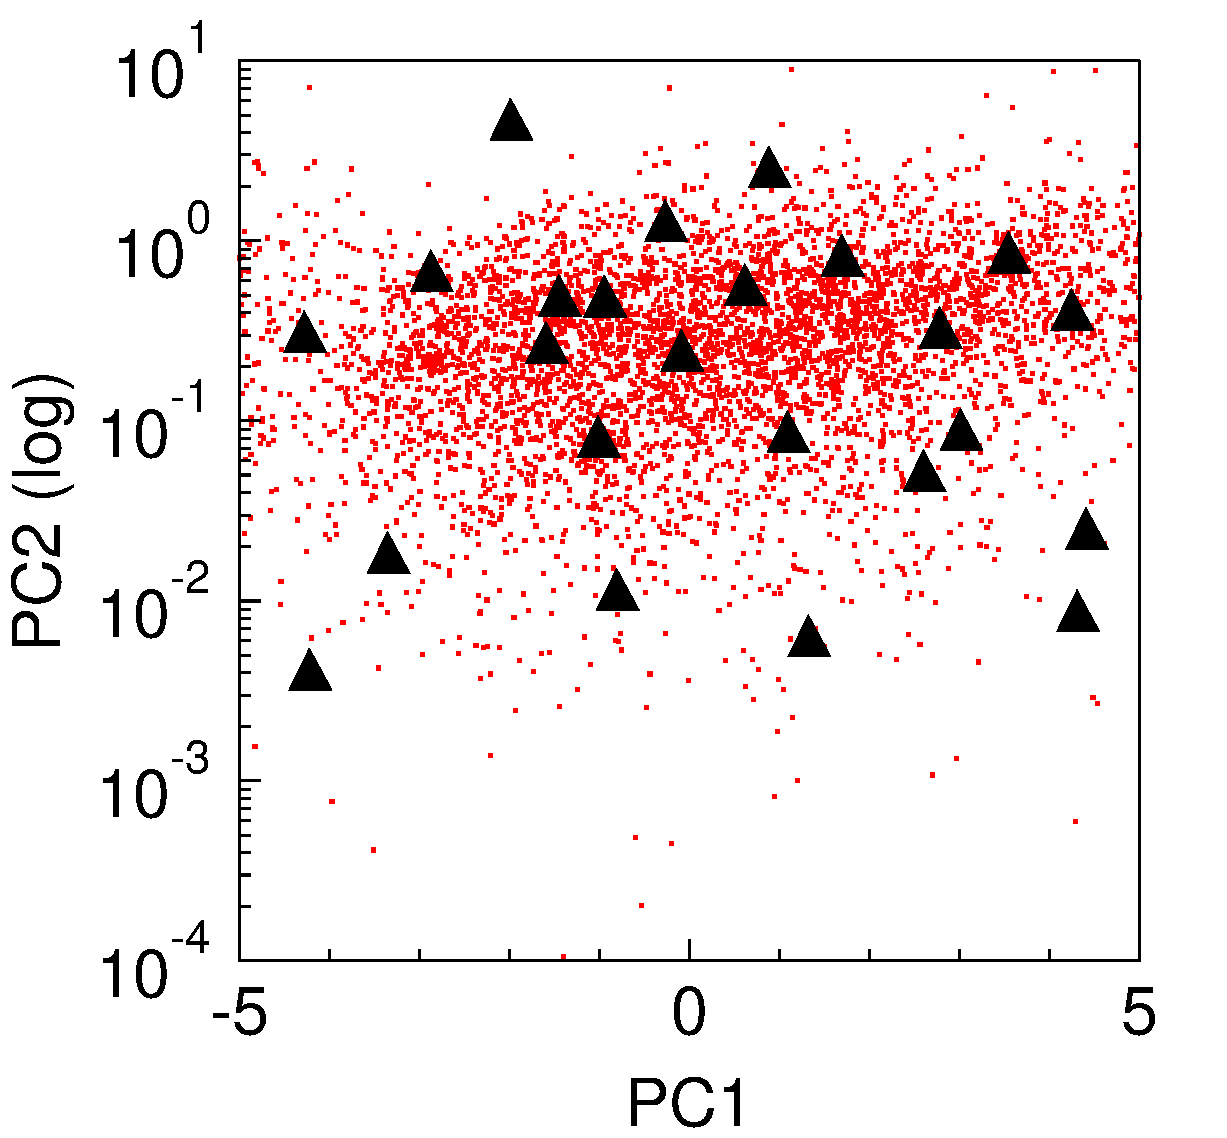
\includegraphics[trim=0 0 0 0, clip, width=.45\columnwidth]{pca}
  \label{fig:pca}
}
\hspace*{15pt}
\subfloat[\small{~\website{www.cnn.com} is a representative webpage from our benchmark suite because it is almost the centroid.}]
{
  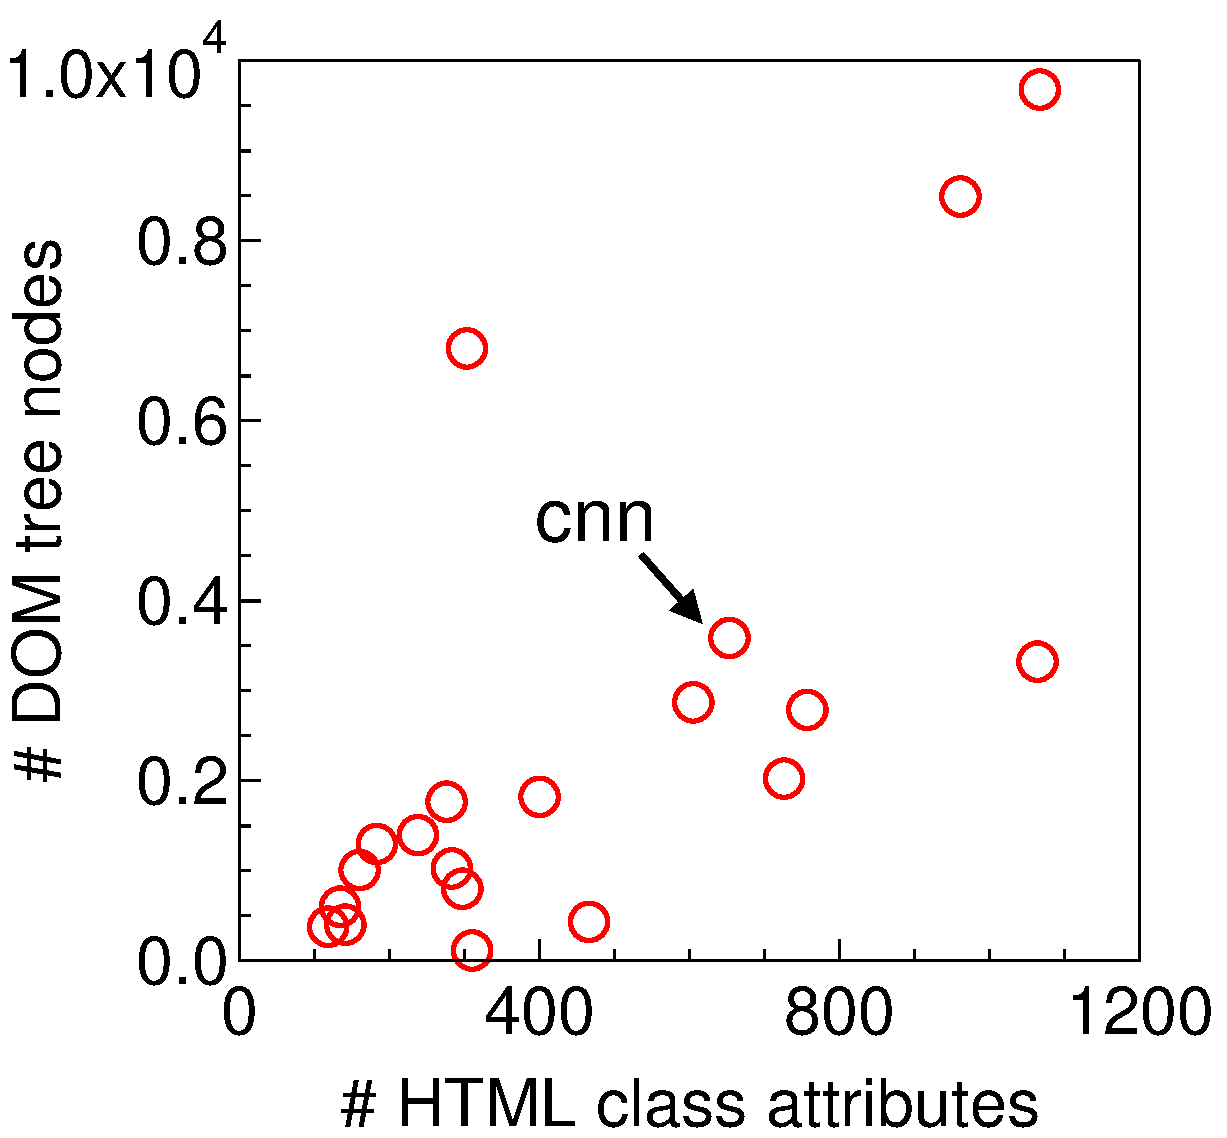
\includegraphics[trim=0 0 0 0, clip, width=.45\columnwidth]{cnn}
  \label{fig:cnn}
} 
\caption{\small Benchmark representativeness analysis.}
\label{fig:bench}
\end{figure}

We consider not only the mobile version of the 12 websites, but also their desktop counterparts. Many mobile users still prefer desktop-version websites for their richer content and experience~\cite{Slocum:2011fk,Bixby:2011uq}. Moreover, many mobile devices, especially tablets, typically load the desktop version of webpages by default. As webpage sizes exceed 1~MB~\cite{Everts:2011kx}, we must study mobile processor architectures that can process more complex content and not just simple mobile webpages.

We study 24 distinct webpages in total. The 24 benchmarked webpages are representative because they capture the webpage variations in both webpage-inherent and microarchitecture-dependent features. To prove this, we performed principal component analysis (PCA), which is a statistical method that reduces the number of inputs without losing generality~\cite{PCA}.  PCA transforms the original inputs into a set of principal components (PC) that are linear combinations of the inputs. In our study, PCA calculates four PCs from about 400 distinct features. These four PCs account for 70\% of the variance across all of the original 10,000 webpages. \Fig{fig:pca} shows the results for two major components, PC1 and PC2. IPC (microarchitecture-dependent feature) is the single most significant metric in PC1, and the number of DOM tree nodes (webpage-inherent feature) is the most significant metric in PC2. The triangular dots represent our webpages. They cover a very large spread of the top 10,000 webpages in the Internet.

\paragraph{Performance Metric} We focus on the initial loading of Web applications. This is because user QoS experience is strongly tied to the initial load time in Web applications. For instance, it is estimated that 79\% of online shoppers will not return to the website with slow load time~\cite{Jacob:2013fk}.

Unless stated otherwise, we define Web application load time as the execution time that elapses until the~\texttt{onload} event is triggered by the Web browser. It is worth noting that during the loading phase (i.e., before the \texttt{onLoad} event is triggered), many Web applications execute JavaScript code such as Ads and analytics. Therefore, our study not only takes into account the initial loading of the webpage, but also includes JavaScript activity that is triggered automatically by Web applications.

\paragraph{Simulators} We assume the x86 instruction set architecture (ISA) for our study. Prior work shows that the ISA does not significantly impact energy efficiency for mobile workloads~\cite{risc-cisc}. Therefore, we believe that our microarchitecture explorations are generally valid across ISAs. We use Marss86~\cite{marss}, a cycle-accurate simulator, in full-system mode to faithfully model all the network and OS activity. Performance counters from Marss86 are fed into McPAT~\cite{mcpat} for power estimation.

%We do our best-effort validation of the simulator by comparing it with an ARM platform because we do not have access to a measurable x86 mobile platform. We use the ODroid XU+E development board~\cite{odroidxue} that hosts the Exynos 5410 SoC as the hardware platform. The Exynos 5410 SoC is known for powering the Samsung's Galaxy S4 smartphone. The Exynos 5410 SoC contains an ARM Cortex-A15 processor. In our measurements, single core Cortex-A15 consumes 1.7~J energy and 2~seconds to load~\website{www.cnn.com}. For comparison, we tune our simulator configurations to best match the microarchitecture parameters of Cortex-A15. The simulation results report 1.2~J and 2.2~seconds for energy consumption and loading time, respective.

\section{Customizing General-Purpose Cores}
\label{sec:arch:customization}

\webcore design is based on general-purpose CPUs to best retain the general-purpose programmability. However, existing general-purpose processors may not be an ideal baseline for \webcore, because they are not uniquely tuned for Web applications. \webcore customizes current designs by exploring a vast design space to properly size key microarchitecture parameters (\Sect{sec:arch:customization:dse}). I derive two major conclusions through the customization process. First, out-of-order designs provide more flexibility for energy versus performance trade-offs than in-order designs (\Sect{sec:arch:customization:core}). Second, a customized out-of-order design configuration still contains two sources of inefficiency--instruction delivery and data feeding--that need to be further mitigated (\Sect{sec:arch:customization:sources}).

\subsection{Design Space Exploration}
\label{sec:arch:customization:dse}

\paragraph{Design Space Specification} We define the set of tunable microarchitectural parameters in \Tbl{tab:dse:para}. We vary the values of functionally related parameters (e.g., issue width and the number of functional units) together to avoid reaching an entirely unbalanced design~\cite{ilp2}. We also do not consider single-issue out-of-order processors, which are known to be energy inefficient~\cite{marginal}. In total, we consider over 3~billion design points.

%!TEX root=../../paper.tex

\begin{table}[p]
\large
\centering
\captionsetup{width=.9\columnwidth}
\caption{Microarchitecture design-space parameters. The first column shows the parameters that are considered in our DSE. The second column shows the metric that the value of each parameter is measured. The $i$::$j$::$k$ in the third column denotes values ranging from $i$ to $k$ at steps of $j$}
\renewcommand*{\arraystretch}{1.4}
\renewcommand*{\tabcolsep}{25pt}
\resizebox{.9\columnwidth}{!}
{
	\begin{tabular}{l l l l l l}
	\toprule[0.15em]
		\bigstrut\textbf{Parameters} & \bigstrut\textbf{Measure} & \bigstrut\textbf{Range}\\
	\midrule[0.05em]
		Issue width				&	count					&	1::1::4	\\
		\# Functional units		&	count					&	1::1::4 \\
		%I-TLB size				&	\#entries				&	8::8::32 \\
		%D-TLB size				&	\#entries				&	8::8::32 \\
		Load queue size			&	\# entries				&	4::4::16 \\
		Store queue size		&	\# entries				&	4::4::16 \\
        Branch prediction size  &   $log_{2}$(\#entries)    &   1::1::10\\
		ROB size				&	\# entries				&	8::8::128 \\
		\# Physical registers	&	\# entries				&	5::5::140 \\
		L1 I-cache size			&	$log_{2}$(KB)			&	3::1::7 \\
		L1 I-cache delay		&	cycles					&	1::1::3 \\
		L1 D-cache size			&	$log_{2}$(KB)			&	3::1::7 \\
		L1 D-cache delay		&	cycles					&	1::1::3\\
		L2 cache size			&	$log_{2}$(KB)			&	7::1::10 \\
		L2 cache delay			&	cycles					&	16,32,64 \\
	\bottomrule[0.15em]
	\end{tabular}
}
\label{tab:dse:para}
\end{table}


We intentionally relax the design parameters beyond the current mobile systems in order to allow an exhaustive design space exploration. For example, we consider up to 128~KB L1 cache design whereas most L1 caches in existing mobile processors are 32~KB in size. Also, since thermal design power (TDP) is important for mobile SoCs, we eliminate overly aggressive designs with more than 2~W TDP.

We assume a fixed core frequency in our design-space exploration. We use 1.6~GHz, a common value in mobile processors~\cite{snapdragon-wiki,exynos-wiki}, to further prune the exploration space. However, because the latency of both the L1 and L2 caches can still vary, we include different cache designs in the exploration space.

We use a constant memory latency to model the memory subsystem because we do not observe significant impact of the memory system on the mobile Web browsing workload. According to hardware measurements on the Cortex-A15 processor using ARM's performance monitoring tool Streamline~\cite{streamline}, the MPKI for the L2 cache across all the webpages is below 5. We observe similar low L2 MPKI, i.e. low main memory pressure, in our simulations. Therefore, we use a simpler memory system to further trim the search space.

\paragraph{Statistical Inference Method} It is not feasible to simulate billions of the design points that we consider simply due to time constraints. Therefore, we leverage the statistical inference technique that trains predictive models using a small number of samples. Such models reflect how different microarchitecture parameters, both individually and collectively, influence performance and power consumption. Statistical inference methods have been used successfully in the past for architecture design-space exploration~\cite{dse,comt}.

In particular, we use linear regression modeling~\cite{RMS} to construct our predictive models. A linear regression model can be formulated as in~\Equ{equ:linear}, where $y$ denotes the response, $x = x_{1},...,x_{p}$ denote \textit{p} predictors, and $\beta = \beta_{0},...,\beta_{p}$ denote corresponding coefficients of each predictor. The \textit{least squares method} is used to solve the regression model by identifying the best-fitting $\beta$ that minimizes the residual sum of squares (RSS)~\cite{ESL}. In our case, the response $y$ is either performance (measured in terms of instruction per cycle, IPC) or power, and the predictors $x_{i}$ are microarchitecture structures listed in \Tbl{tab:dse:para}.

\begin{equation}
       y = \beta_0 + \sum_{i=1}^{p} x_i \beta_i
\label{equ:linear}
\end{equation}

We find that 2,000 \textit{uniformly at random} (UAR) samples of microarchitecture configurations from the design space are sufficient in our case to construct robust models. We also obtain 500 additional UAR samples from the cache design space (both L1 and L2) to reinforce the credibility of instruction and data cache design predictions. We perform cross-validation of the model (i.e., we partition a sample dataset into complementary subsets, and perform analysis on one subset and validate the analysis on the other subset), and then obtain additional samples from the design space for full evaluation.

In order to derive general conclusions about the design space and optimize for the common case, in this section we present only our in-depth analysis for the representative website \website{www.cnn.com}. ~\Fig{fig:cnn} compares~\website{www.cnn.com} with other webpages to demonstrate that it is indeed representative of the other benchmarked webpages. The $x$-axis and $y$-axis represent the number of DOM tree nodes and the number of~\textsf{class} attributes in HTML. These are the two webpage characteristics that are most correlated with a webpage's load time and energy consumption~\cite{big-little}. As the figure shows,~\website{www.cnn.com} is roughly the centroid of the benchmarked webpages, and thus we use it as a representative webpage for the common case.

We construct predictive models for out-of-order and in-order design space separately because microarchitecture structures have different impact on performance and power in in-order and out-of-order pipelines. In general, the out-of-order models' error rates are below 6.0\%. The in-order models (not shown) are more accurate because of their simpler design. On average, the in-order performance and power models' errors are within 5\% and 2\%, respectively.

\begin{figure}[t]
  \centering
  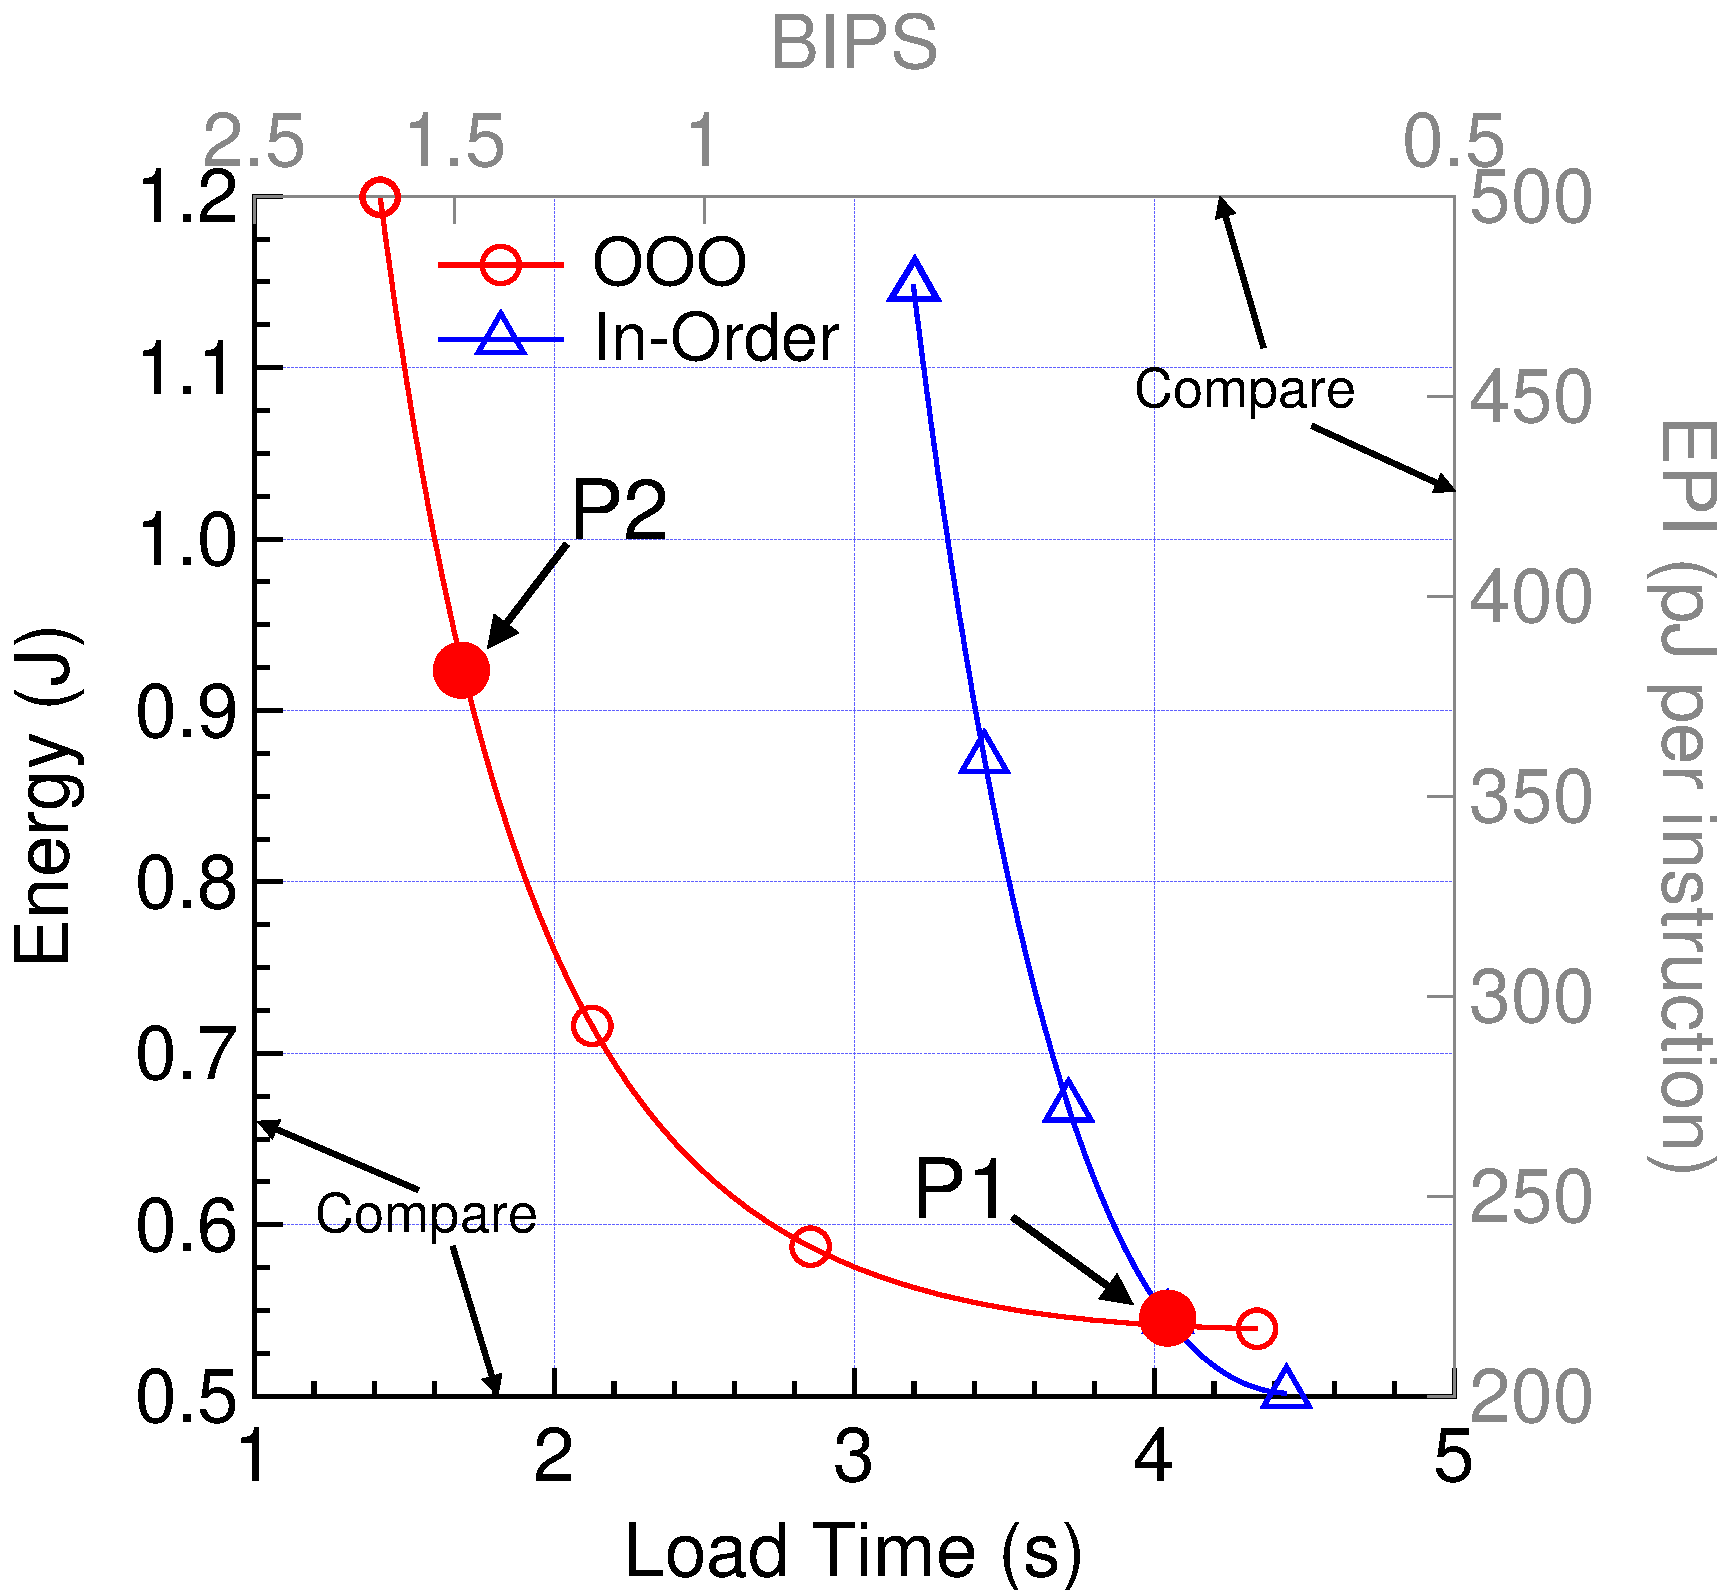
\includegraphics[trim=0 0 0 0, clip, width=.6\columnwidth]{ivso}
  \caption{In-order versus out-of-order Pareto optimal frontiers.}
  \label{fig:ivso}
\end{figure}

\subsection{In-order vs. Out-of-order Design Space Exploration}
\label{sec:arch:customization:core}

Design space exploration helps customization at the ``macro-architecture'' level, i.e., determining between in-order and out-of-order designs. We understand the difference between in-order and out-of-order design space by examining their Pareto optimal frontiers. Design points on a Pareto optimal frontier reflect different optimal design decisions given specific performance/energy targets. The Pareto-optimal is more general than the (sometimes overly specific) $EDP$, $ED^{2}P$ metrics, etc. Design configurations optimized for such metrics have been known to correspond to different points on the Pareto-optimal frontier~\cite{marginal}. \Fig{fig:ivso} shows the Pareto-optimal frontiers of both in-order and out-of-order designs between energy and performance. We use energy per instruction (EPI) for the energy metric, and million instructions per second (MIPS) as the performance metric. 

We make two important observations from \Fig{fig:ivso}. First, the out-of-order design space offers a much larger performance range ($\sim$1~BIPS between markers P1 and P2, see top $x$-axis) than the in-order design space (\textless~0.5~BIPS), which reflects the out-of-order's flexibility in design decisions. Second, the out-of-order design frontier is flatter around the 4-second webpage load time range (see marker P1) than in the in-order design, which indicates that the out-of-order design has a much lower marginal energy cost. The observation indicates that processor architects can make design decisions based on the different performance goals without too much concern about the energy budget. In contrast, the in-order design space quickly enters the region of diminishing returns (i.e., sharp increase in energy consumption) as we push toward webpage load times that are less than 4 seconds. In other words, the in-order design has a low marginal performance value (or equivalently high marginal cost of energy).

%\Fig{fig:ivso} shows the Pareto optimal frontiers of the in-order and out-of-order design space. We observe that the in-order design space has a narrow performance range of 1~second, whereas the out-of-order space covers a 4~second performance range. The performance range contrast indicates that out-of-order designs can more flexibly balance performance with energy and, therefore, are better design baselines for mobile Web applications.

\begin{figure}[t]
  \centering
  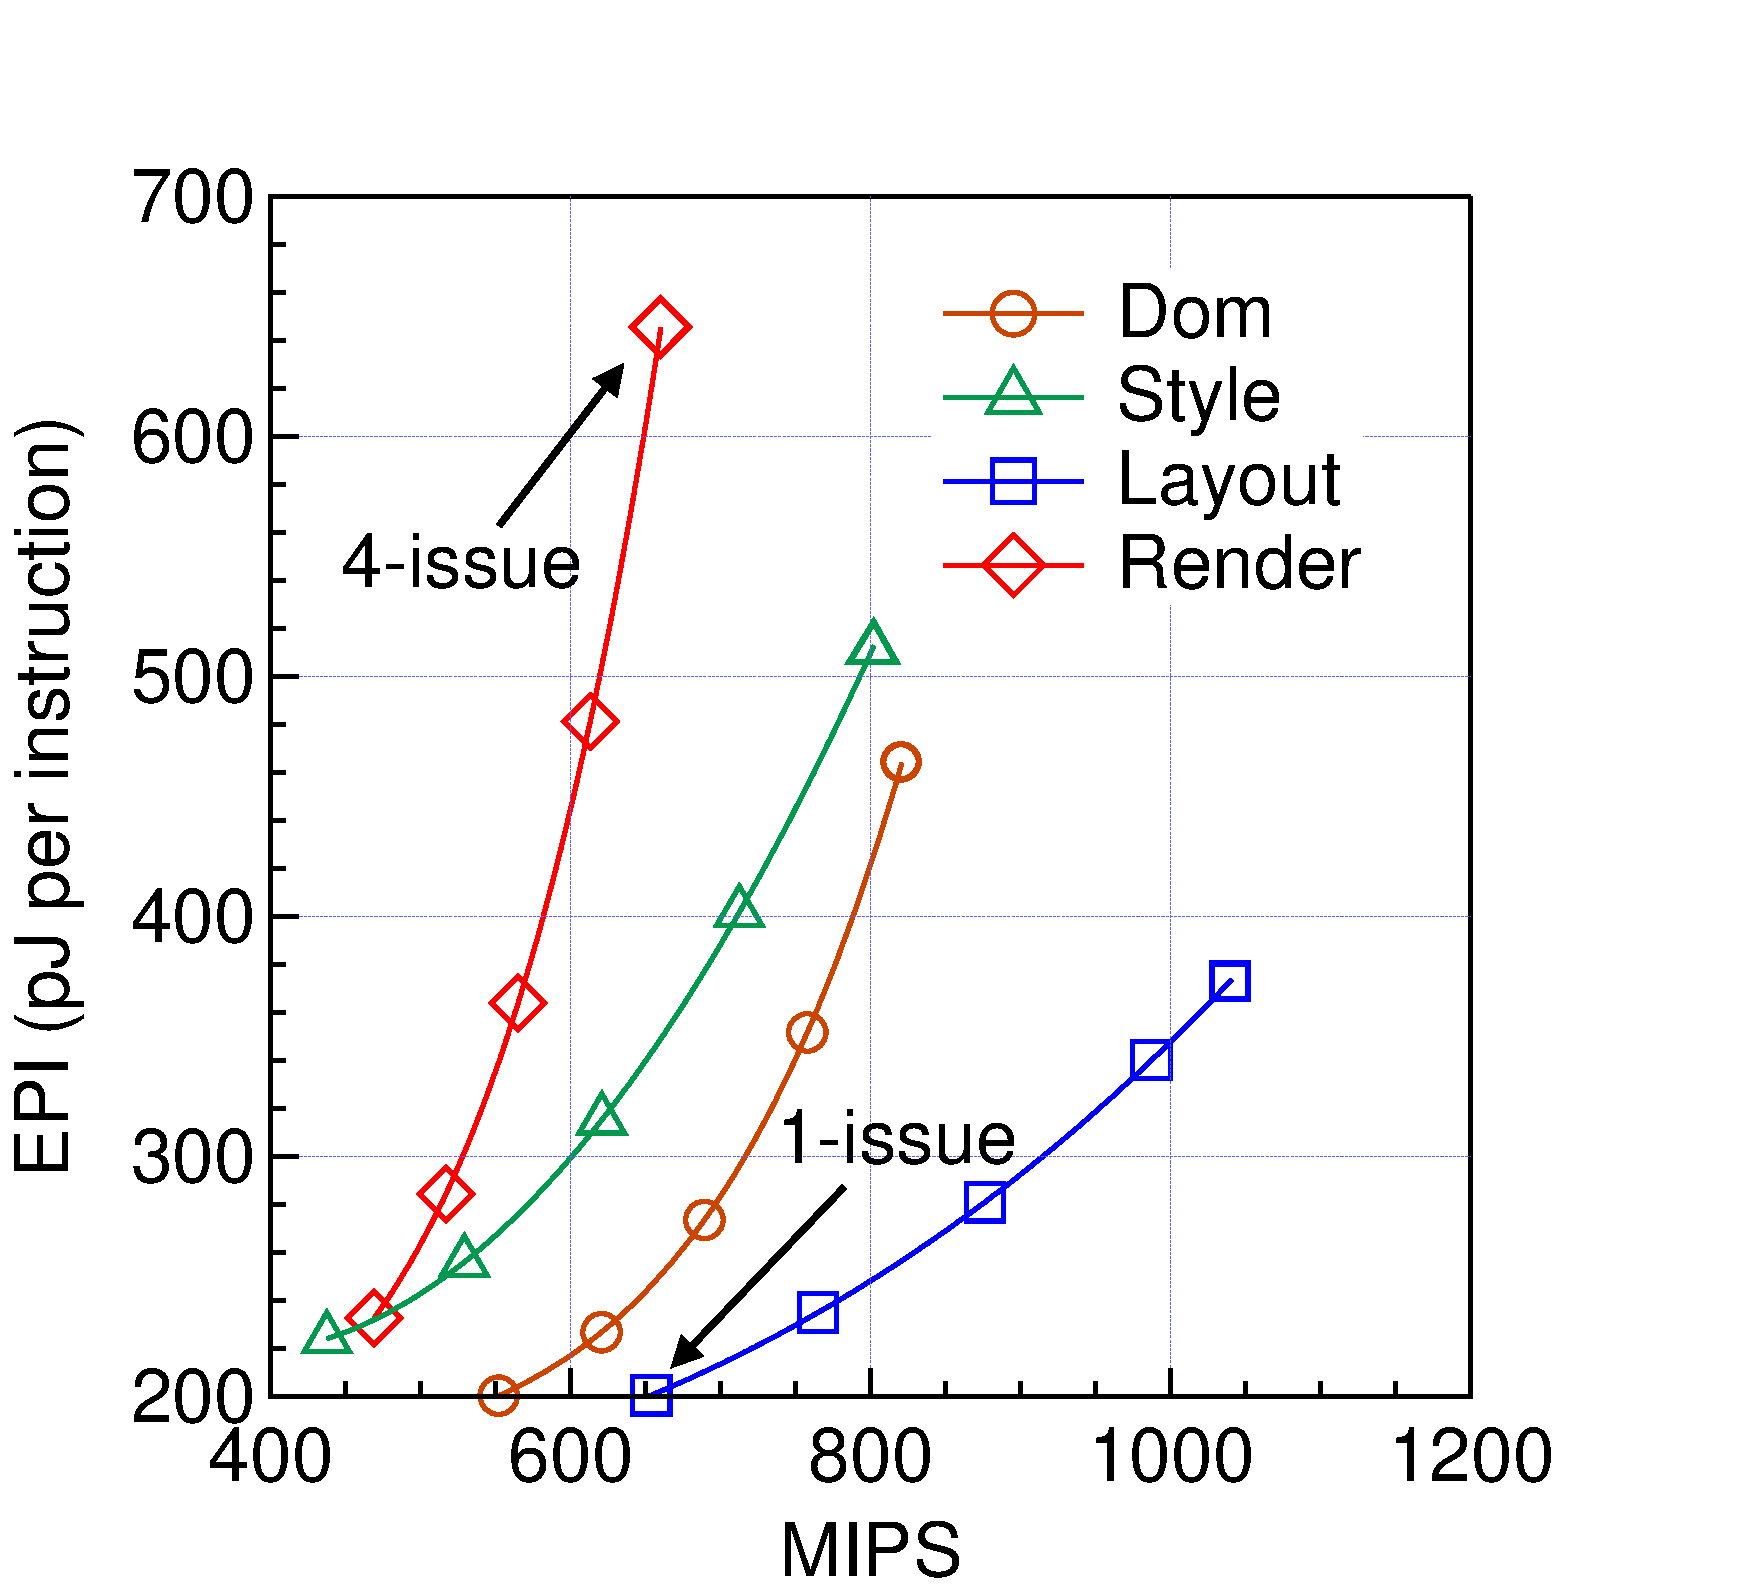
\includegraphics[trim=0 0 0 0, clip, width=.6\columnwidth]{pareto_io}
  \caption{In-order Pareto optimal frontier for each kernel.}
  \label{fig:pareto_io}
\end{figure}

\begin{figure}[t]
  \centering
  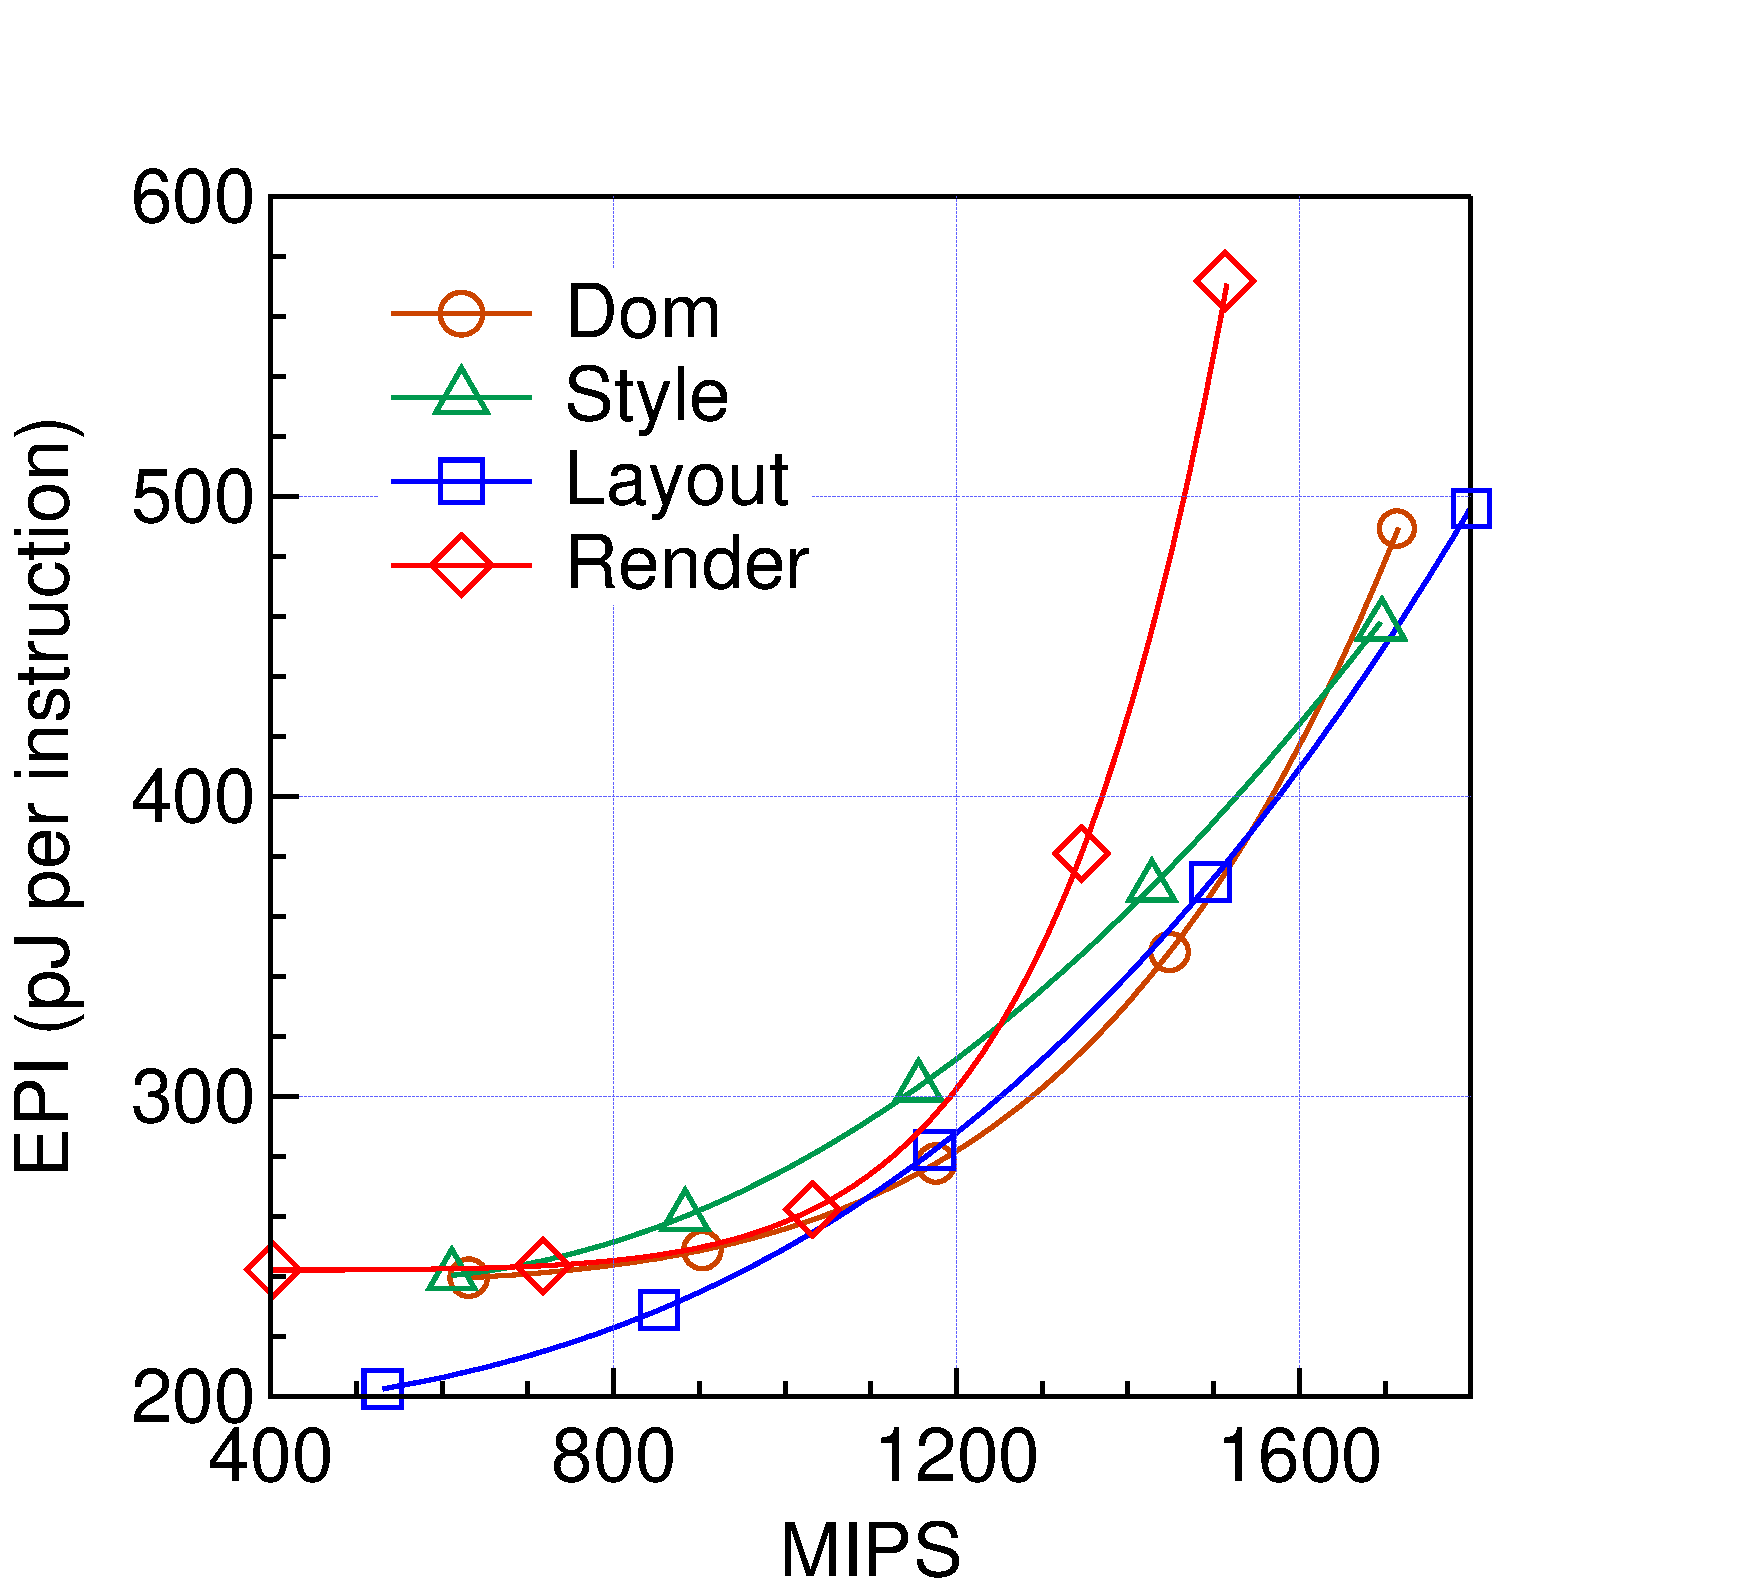
\includegraphics[trim=0 0 0 0, clip, width=.6\columnwidth]{pareto_ooo}
  \caption{Out-of-order Pareto optimal frontier for each kernel.}
  \label{fig:pareto_ooo}
\end{figure}

To understand the difference behind the in-order versus out-of-order designs, we study the kernel behaviors in Web applications. There are four important computation kernels in executing a Web application: i.e.,~\textit{Dom}, \textit{Style}, \textit{Layout}, and \textit{Render}. They contribute to about 75\% of the webpage load time and energy consumption.~\Fig{fig:pareto_io} and~\Fig{fig:pareto_ooo} show the Pareto optimal frontiers of the in-order and out-of-order design space for each kernel. We find that the kernel variance in the in-order designs is more pronounced than in the out-of-order designs. As we push toward more performance in the in-order design space, some kernels stop scaling gracefully on the energy-versus-delay curve, and eventually become a performance bottleneck. Overall, in-order designs have low marginal performance value with high marginal energy cost~\cite{marginal}. In contrast, out-of-order cores can cover the variances across the different kernels through complex execution logic and, therefore, provide wider performance and energy trade-off range.

\subsection{Sources of Inefficiency}
\label{sec:arch:customization:sources}

DSE also helps customization at the microarchitecture level. We examine microarchitectural parameters of two out-of-order Pareto optimal designs: P1 and P2 in \Fig{fig:ivso}. They represent designs optimized for different performance and energy targets. P1 is optimized for minimal energy consumption in the out-of-order space. P2 is a high-performance design with a performance of 1500 MIPS (million instructions per second). \Tbl{tab:dse:ednp} summarizes the microarchitecture configurations of the two designs. For comparison purposes, it also lists the same parameters for ARM Cortex-A15, which represents today's high-end mobile CPU.

%!TEX root=../../paper.tex

\begin{table}[p]
\large
\centering
\captionsetup{width=.9\columnwidth}
\caption{Microarchitecture configurations for P1 and P2 in
\Fig{fig:ivso}. They represent different energy-delay trade-offs. For comparison purpose, we also show the parameters for ARM Cortex-A15, whose information is gather from measurements using the 7-Zip LZMA Benchmark~\cite{7cpu-a15} and ARM's public presentation~\cite{a15-slide}.}
\renewcommand*{\arraystretch}{1.4}
\renewcommand*{\tabcolsep}{15pt}
\resizebox{.9\columnwidth}{!}
{
	\begin{tabular}{l c c c}
	\toprule[0.15em]
        ~      & \bigstrut\textbf{P1} & \bigstrut\textbf{P2} & \bigstrut\textbf{Cortex-A15}\\
	\midrule[0.05em]
        Issue width						&	1		&	3	&	3	\\
        \# Functional units				&	2		&	3	&	8	\\
        Load queue size (\# entries)		&	4		&	16	&	16	\\
        Store queue size (\# entries)	&	4		&	16	&	16	\\
        BTB size (\# entries)   &       1024    &       128 &   64       \\
        ROB size (\# entries)			&	128		&	128	&	40+	\\
        \# Physical registers			&	128		&	128	&	?	\\
        L1 I-cache size (KB)				&	64		&	128	&	32	\\
        L1 I-cache delay (cycles)		&	1		&	2	&	?	\\
        L1 D-cache size (KB)				&	8		&	64	&	32	\\
        L1 D-cache delay (cycles)		&	1		&	1	&	4	\\
        L2 cache size (KB)				&	256&	1024	&	512\textasciitilde4096	\\
        L2 cache delay (cycles)			&	16		&	16	&	21	\\
	\bottomrule[0.15em]
    \end{tabular}
}
\label{tab:dse:ednp}
\end{table}


By comparing P1 and P2 with Cortex-A15, we find two major sources of inefficiencies in general-purpose processors: instruction delivery and data feeding. First, current mobile processors have a small L1 instruction cache that is typically 32~KB in size. However, the two Pareto optimal designs require a 64~KB to 128~KB instruction cache to alleviate the pressure on instruction delivery in mobile Web applications. The pathological front-end behavior mainly stems from the large instruction footprint and the prevalence of the irregular control flow path~\cite{BBench}.

Second, the high-performance design P2 also necessitate a 64~KB data cache, doubling the typical L1 data cache size in current mobile CPUs. The need for a large data cache mainly stems from the large working set size on principal data structures (e.g., the DOM tree) during webpage processing. For example, profiling results show that the average data reuse distance for DOM tree accesses is 4~KB (excluding other memory operations interleaved with DOM accesses). The large data cache leads to excessive energy consumption and needs to be optimized.

\section{Style Resolution Unit}
\label{sec:arch:sru}

Unusual design parameters in a customized processor tuned for the mobile Web workload indicate that instruction delivery and data feeding are critical to guarantee high performance while still being energy efficient. I propose specialized hardware mechanisms to mitigate the instruction delivery and data feeding inefficiencies in the customized out-of-order core designs. In particular, I introduce two new hardware structures: a Style Resolution Unit (SRU) and a Browser Engine Cache (BEC). This section focuses on the SRU and the next section focuses on the BEC.

The SRU is an accelerator for the critical \textit{Style} kernel within the Web browser rendering engine. The SRU design is based on the observation that the \textit{Style} kernel has abundant fine-grained parallelism that is hidden in a software implementation but can be captured by a dedicated hardware structure~(\Sect{sec:sru:motivation}). To exploit the inherent fine-grained parallelism, the SRU employs a multi-lane parallel architecture, which greatly reduces the instruction delivery overhead. To reduce the data feeding pressure, the SRU is tightly coupled with a small scratchpad memory that brings operands closer to the SRU~(\Sect{sec:sru:hw}). To maintain general-purpose programmability, these new hardware structures are accessed via a set of high-level language APIs. The APIs are implemented through a runtime library with only slight modification to the current browser implementation~(\Sect{sec:sru:sw}).

%\Fig{fig:framework} shows an overview of our proposed optimization framework. Overall, the hardware supports fast and energy-efficient execution and data communication, and the library hides the hardware complexity, manages the hardware executions, and eases the software development effort.

\subsection{Motivation}
\label{sec:sru:motivation}

Optimizing the \textit{Style} kernel would improve the overall energy efficiency the most for the following reasons. The~\textit{Style} kernel is the most time-consuming task in the rendering engine. In our profiling, it consumes 35\% of the total rendering engine execution time. it also dominates the energy consumption by consuming 40\% of the total energy.

In order to mitigate the instruction delivery and data communication overhead of the~\textit{Style} kernel, we propose a special functional unit called the~\textit{Style Resolution Unit} (SRU) that is tightly coupled with a small scratchpad memory. The SRU exploits fine-grained parallelism to reduce the amount of instructions and potential divergences. The scratchpad memory reduces data communication pressure by bringing operands closer to the SRU.

\begin{figure}[t]
\centering
\captionsetup{width=\columnwidth}
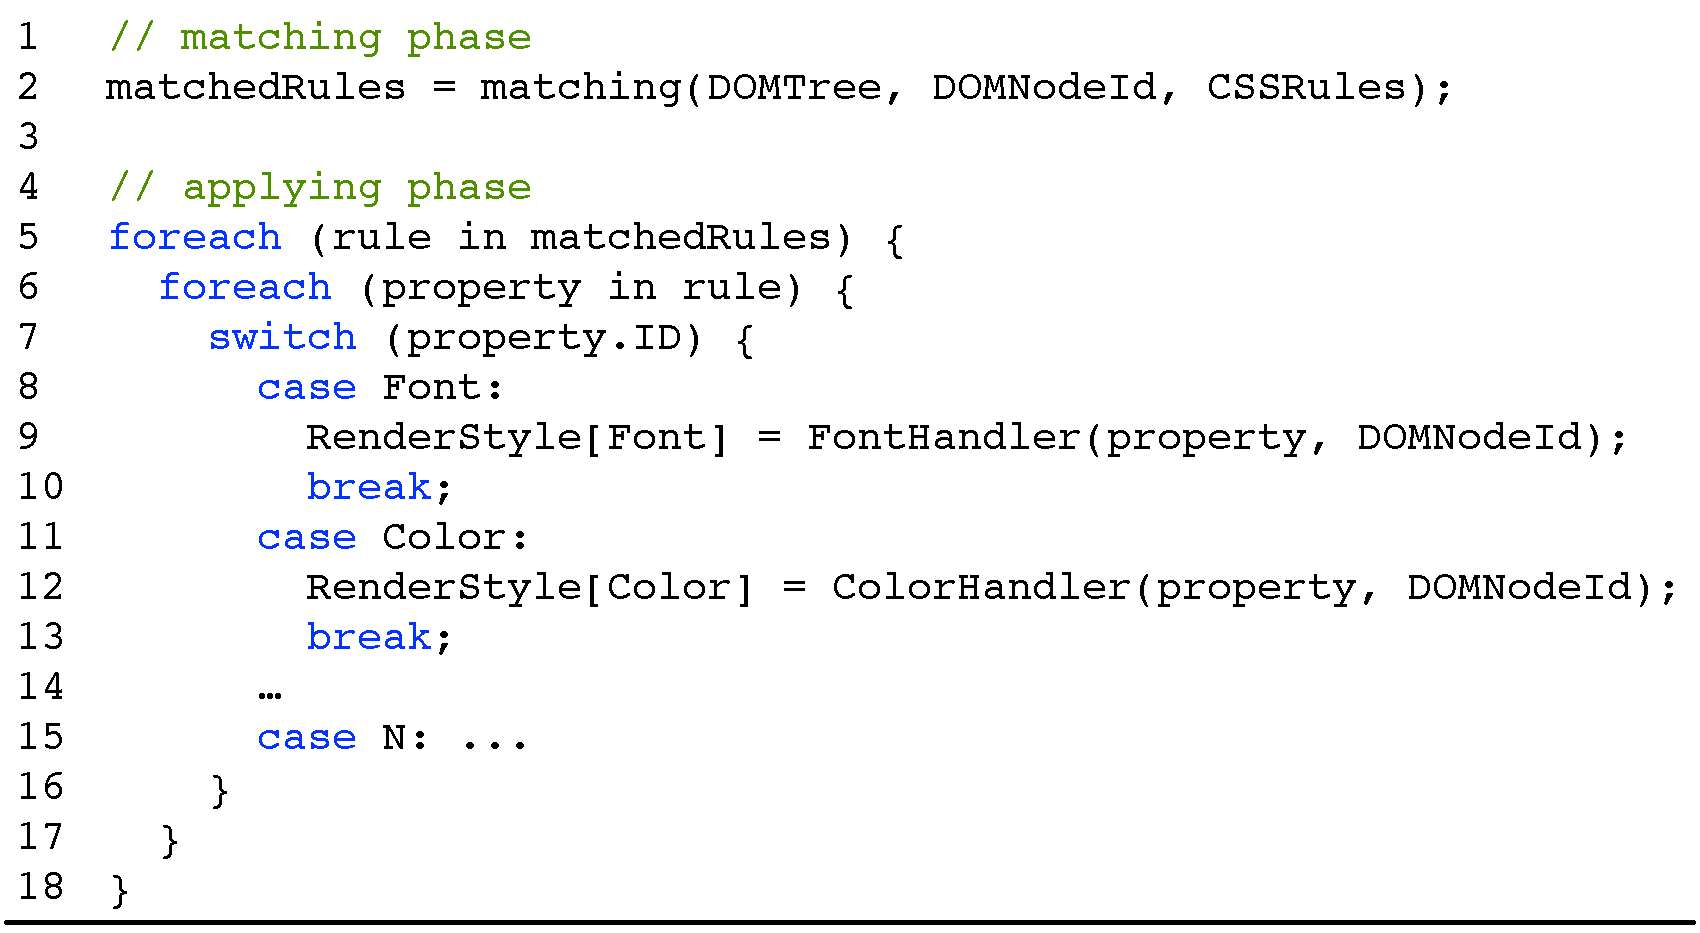
\includegraphics[trim=0 0 0 0, clip, width=\columnwidth]{style-code}
\caption{\small{Pseudo-code of the \textit{Style} kernel. It consists of a matching phase and an applying phase. SRU accelerates the applying phase, which takes about two-thirds of the \textit{Style} kernel execution time.}}
\label{fig:style-code}
\end{figure}

The \textit{Style} kernel consists of two phases: a matching phase and an applying phase. \Fig{fig:style-code} shows the pseudo-code of the two phases. Previous work~\cite{zoomm,ParallelBrowser} focuses on parallelizing the matching phase. However, in our profiling, we find that the applying phase takes nearly twice as long to execute as the matching phase. Therefore, we focus on the applying phase. The applying phase takes in a set of CSS rules (\texttt{matchedRules}) as input, iterates over each rule in the correct cascading order~\cite{cascading} to calculate each style property's final value (e.g., the exact-color RGB values, font width pixels). The final values are stored back to the Render tree (the \texttt{RenderStyle} array).

The key observation we make in the applying phase is that there are two types of inherent parallelism: ``rule-level parallelism'' (RLP) and ``property-level parallelism'' (PLP). Improving the energy efficiency of the~\textit{Style} kernel requires us to exploit both forms of parallelism in order to reduce the control-flow divergence and data communication overheads. Our profiling results indicate that both control flow and memory instructions put together constitute 80\% of the total instructions that are executed within the \textit{Style} kernel.

RLP comes from the following. In order to maintain the correct cascading order, each rule contained in the input data structure must be sequentially iterated from the lowest priority to the highest, so that the higher-priority rules can override the lower-priority rules. However, in reality, we could speculatively apply the rules with different priorities in parallel, and select the one with the highest priority. PLP follows RLP. Each rule has multiple properties, and each property is examined by the engine to set the corresponding data field in the Render tree according to its property ID. Because properties are independent of one another, handling of their processing routines can be dealt with in parallel.

\subsection{Hardware Design}
\label{sec:sru:hw}

We propose a parallel hardware unit that exploits both RLP and PLP, called the Style Resolution Unit. The SRU aggregates enough computations to reduce control-flow divergences and increase arithmetic intensity. It is accompanied by data storage units for both input and output. Note that it is not easy to exploit software-level parallelism for PLP and RLP because of the complex control flow, memory aliasing, and severe loop-carried dependencies.

\begin{figure}[t]
\centering
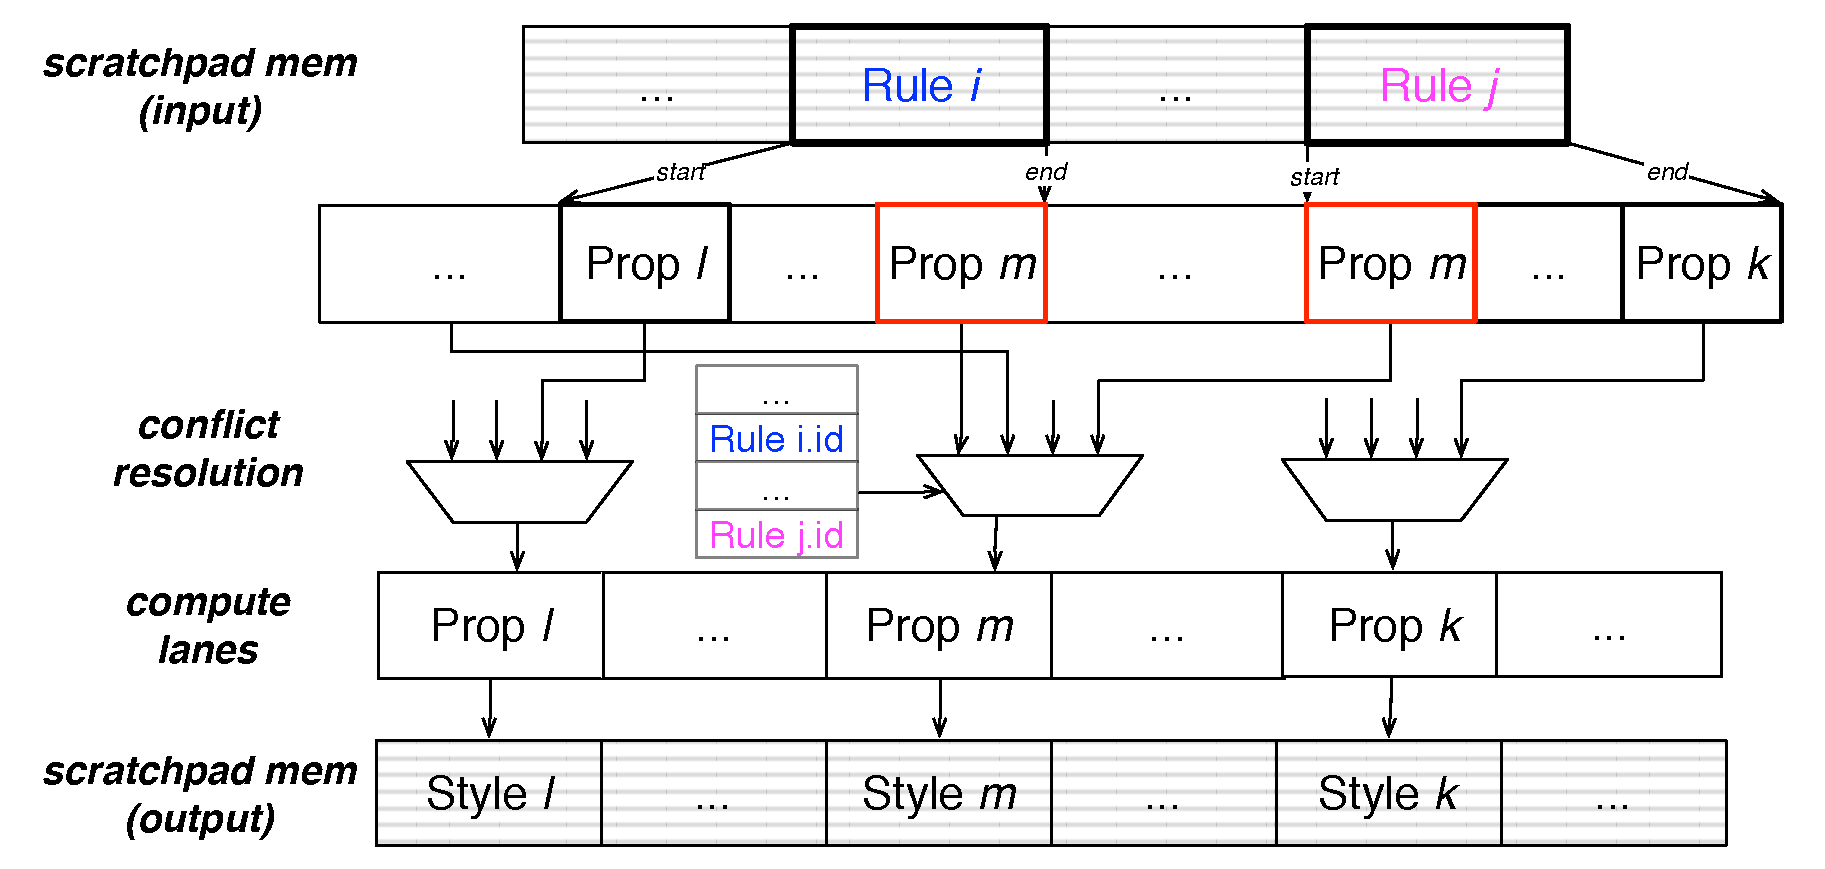
\includegraphics[trim=0 0 0 0, clip, width=\columnwidth]{sru}
\caption{\small{SRU coupled with scratchpad memories.}}
\label{fig:sru}
\end{figure}

In addition, we noticed that the input to the applying phase, \texttt{matchedRules}, is an intra-kernel shared data structure between the matching and applying phases. Storing such short-lived data into the memory hierarchy, and accessing it through traditional load and store instructions, results in slow computation. It also wastes energy. Therefore, we provide a scratchpad memory for the input. Similarly, we store the output structure (i.e., \texttt{RenderStyle}) in a separate scratchpad memory.

\Fig{fig:sru} shows the structure of the SRU with scratchpad memory for input and output data. SRU has multiple lanes, with each lane dealing with one CSS property. Assume Rule~$i$ and Rule~$j$ are two rules from the input that are residing in the scratchpad memory. Rule~$i$ has higher priority than Rule~$j$. Prop~$l$ and Prop~$m$ are two properties in Rule~$i$. Similarly, Rule~$j$ has properties Prop $k$ and Prop $m$. Prop~$l$ and Prop~$k$ can be executed in parallel using different SRU lanes because they do not conflict with each other. However, Prop~$m$ is present in both rules, and as such it causes an SRU lane conflict, in which case the MUX selects the property from the rule with the highest priority, which in our example is Rule~$i$.

%At execution time upon reaching the \texttt{Style\_Apply()} API that programmers use for trigerring the applying phase, the runtime layer copies all the matched rules into the scratchpad memory before the applying phase starts, issue instructions to the SRU, and copies the final style values back to the memory once SRU finishes.

\paragraph{Design Considerations} A hardware implementation can have only a fixed amount of resources. Therefore, the number of SRU lanes and the size of the scratchpad memory is limited. Prior work~\cite{big-little} shows that the number of matched CSS rules and the number of properties in a rule can vary from one webpage to another. As such, a fixed design may overfeed or underfeed the SRU if the resources are not allocated properly.

\begin{figure}[t]
\centering
\subfloat[\small{RLP analysis.}]
{
  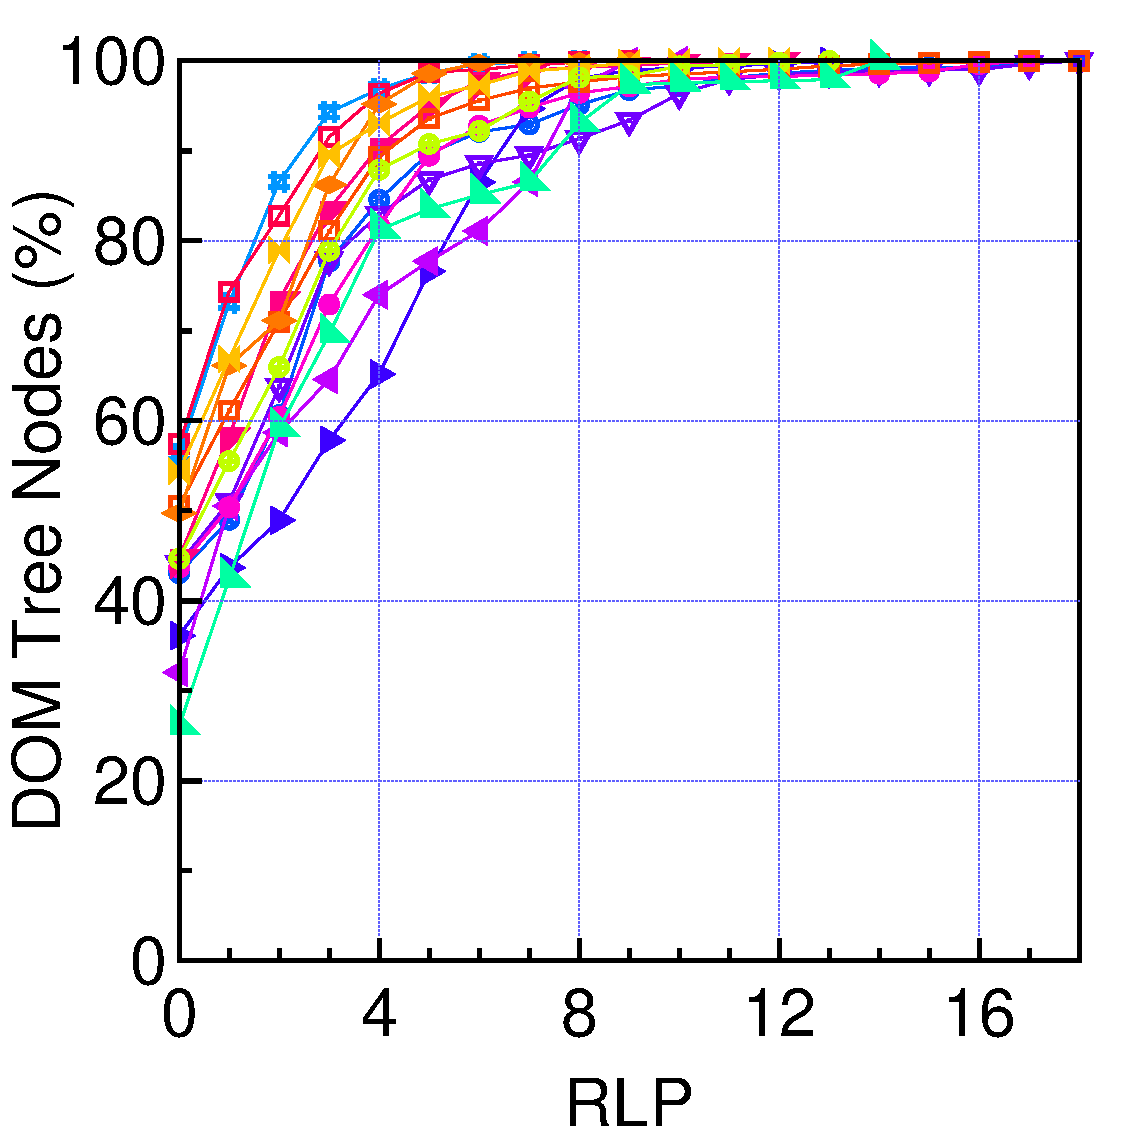
\includegraphics[trim=0 0 0 0, clip, width=.45\columnwidth]{rlp}
  \label{fig:rlp}
}
\hspace*{15pt}
\subfloat[\small{CSS property analysis.}]
{
  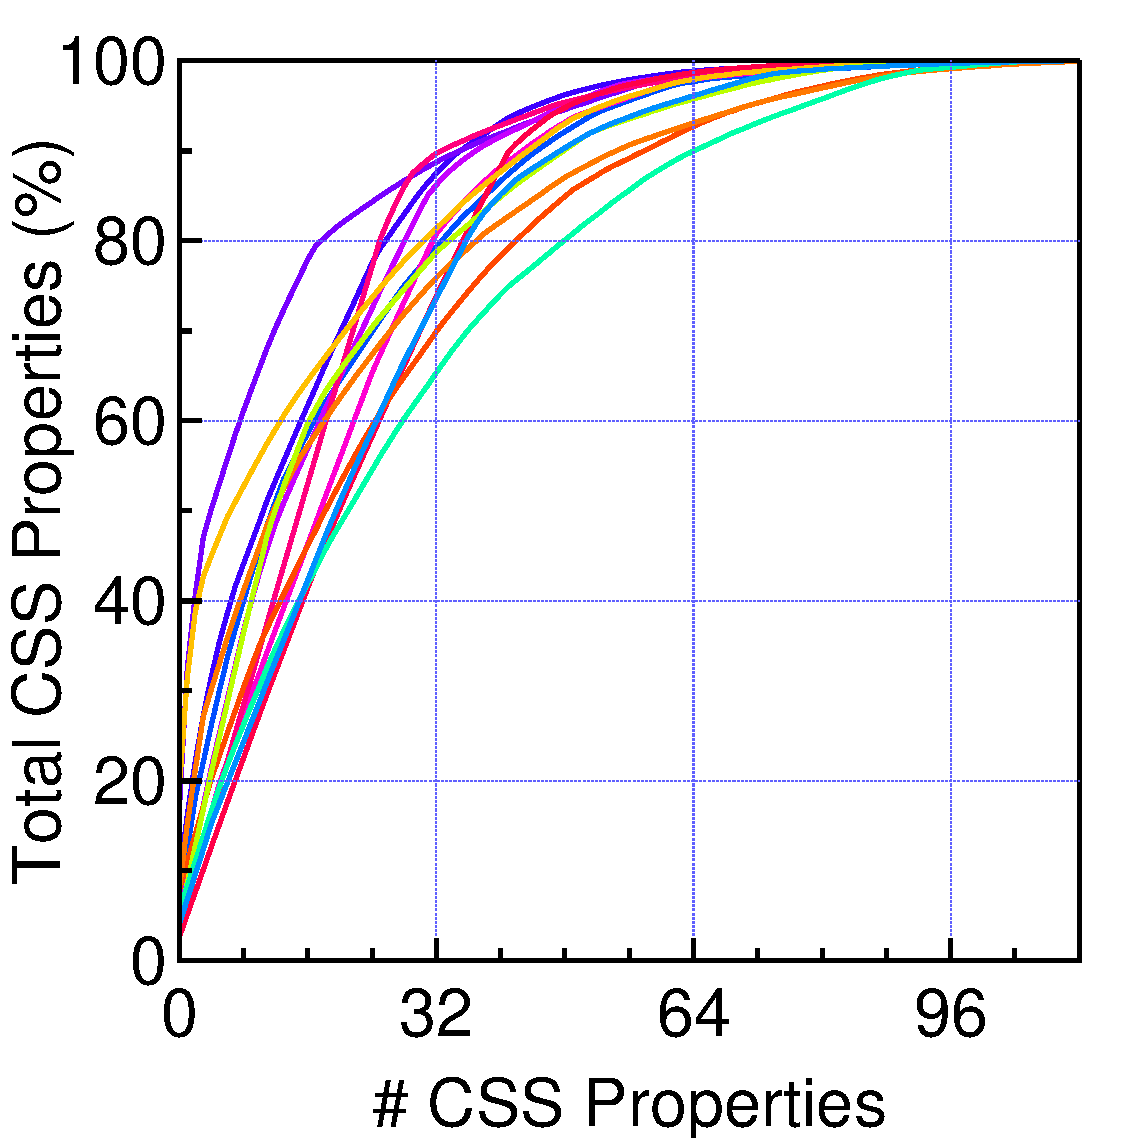
\includegraphics[trim=0 0 0 0, clip, width=.45\columnwidth]{plp}
  \label{fig:plp}
} 
\caption{\small Analysis of RLP and CSS properties across webpages.}
\label{fig:para}
\end{figure}

We profile the webpages to determine the appropriate amount of resource allocation required for the SRU. Profiling indicates that 90\% of the time, the RLP is below or equal to 4 (\Fig{fig:rlp}). Therefore, our design's scratchpad memory only stores up to four styles. Similarly, 32 hot CSS properties cover about 70\% of the commonly used properties (\Fig{fig:plp}). Thus, we implement a 32-wide SRU where each lane handles one hot CSS property. Due to these considerations, the input and output scratchpad memories are each 1~KB in size.

Furthermore, not all of the properties are delegated to the SRU. For example, some style properties require information on the parent and sibling nodes. To avoid complex hardware design for recursions and loops with unknown iterations, we do not implement them in our SRU prototype. The runtime library performs these checks, which we discuss later in~\Sect{sec:sru:sw}. Despite the trade-offs we make, about 72.4\% of the style rules across all the benchmarked webpages can utilize the SRU.  

\subsection{Software Support and Programmability}
\label{sec:sru:sw}

The SRU can be accessed via a small set of instruction extensions to the general-purpose ISA. In order to abstract the low-level details away from application developers, we provide a set of library APIs in high-level languages. Application developers use the APIs without knowing the existence of the specialized hardware. It is important to notice that these software APIs are used by Web browser rendering engine developers rather than high-level Web application developers. WebCore does not affect the programming interface of Web application developers, and therefore has no impact on the Web application development productivity.

\begin{figure}[h]
\centering
\captionsetup{width=.8\columnwidth}
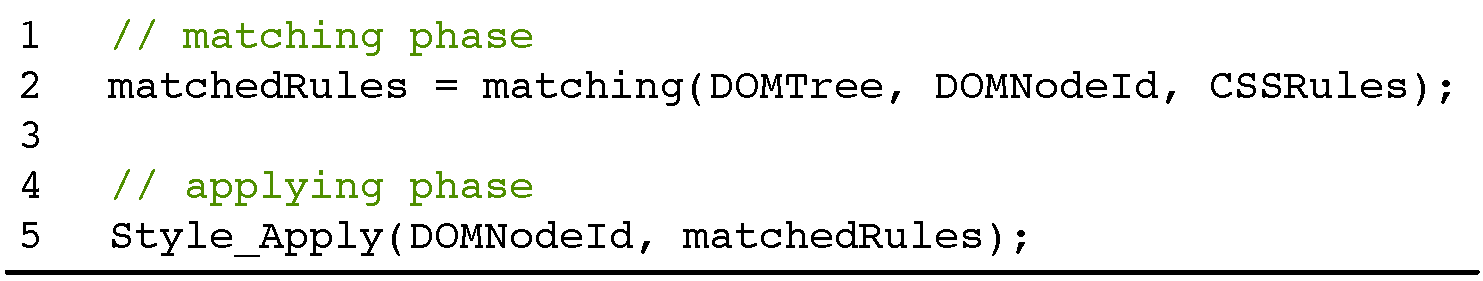
\includegraphics[trim=0 0 0 0, clip, width=.9\columnwidth]{style-code-sru}
\caption{\small{Pseudo-code of the \textit{Style} kernel with the new API.}}
\label{fig:style-code-sru}
\end{figure}

Programmers trigger the style resolution task by issuing a~\texttt{Style\_Apply(Id, Rules)} API, in which \texttt{Id} represents a DOM tree node ID and \texttt{Rules} represents matched CSS rules produced by the matching phase. \Fig{fig:style-code-sru} illustrates the pseudo-code of the \textit{Style} kernel using the provided API. Comparing against the original code in \Fig{fig:style-code}, we notice that the matching phase is not changed while the applying phase is greatly simplified with the \texttt{Style\_Apply} API.

One key task of this API implementation is to examine all the CSS properties of a particular DOM node because not all the CSS properties are implemented in the SRU (as discussed in~\Sect{sec:sru:hw}). For properties that can be offloaded to the SRU, the API implementation loads related data into the SRU's scratchpad memory. For those ``unaccelerated'' properties, the runtime creates the necessary compensation code. Specifically, we propose relying on the existing software implementation as a fail-safe fallback mechanism. Once the style resolution results are generated, the results can be copied out to the output scratchpad memory.

\section{Browser Engine Cache}
\label{sec:cache}

To further improve the energy-efficiency of date feeding, we propose the browser engine cache. It is based on the observation that Web applications' accesses to principal data structures, such as the DOM tree and the Render tree, exhibit heavy data reuse and predictable access pattern~(\Sect{sec:cache:motivation}). Based on such an observation, the browser engine cache uses a small hardware memory structure coupled with a lightweight software-based cache management layer to provide energy-efficient data access~(\Sect{sec:cache:hw}). In addition, similar to SRU, we also provide a set of high-level language APIs that allow Web browser developers to easily access the browser engine cache~(\Sect{sec:cache:sw}).

\subsection{Motivation}
\label{sec:cache:motivation}

\begin{figure}[t]
\centering
\subfloat[\small{DOM node reuse behavior.}]
{
	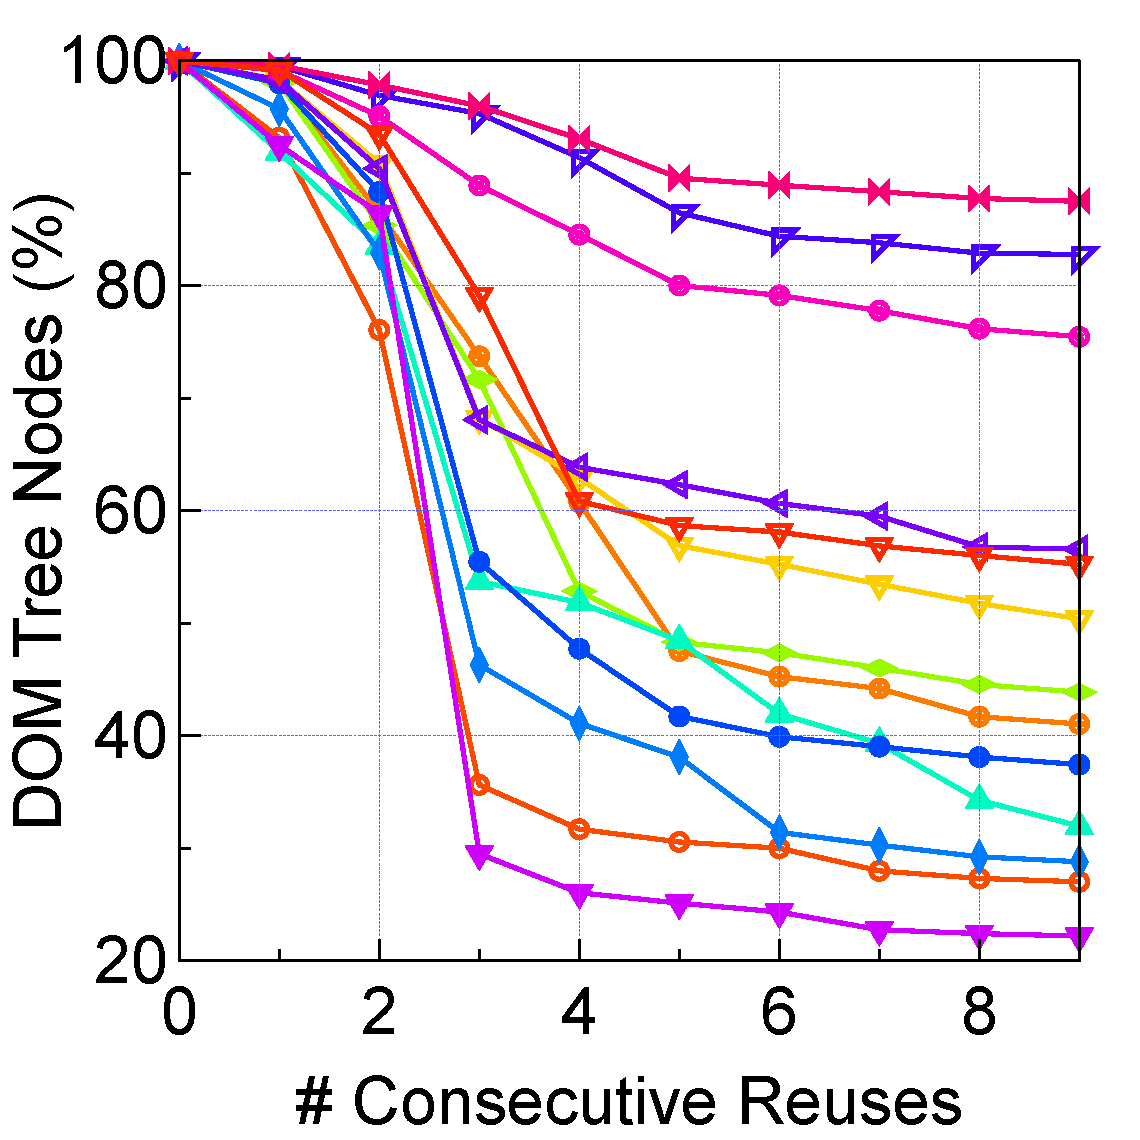
\includegraphics[trim=0 0 0 0, clip, width=.45\columnwidth]{cdf-con-reuse}
	\label{fig:con-reuse}
}
\hspace*{15pt}
\subfloat[\small{DOM node access hit rate.}]
{
	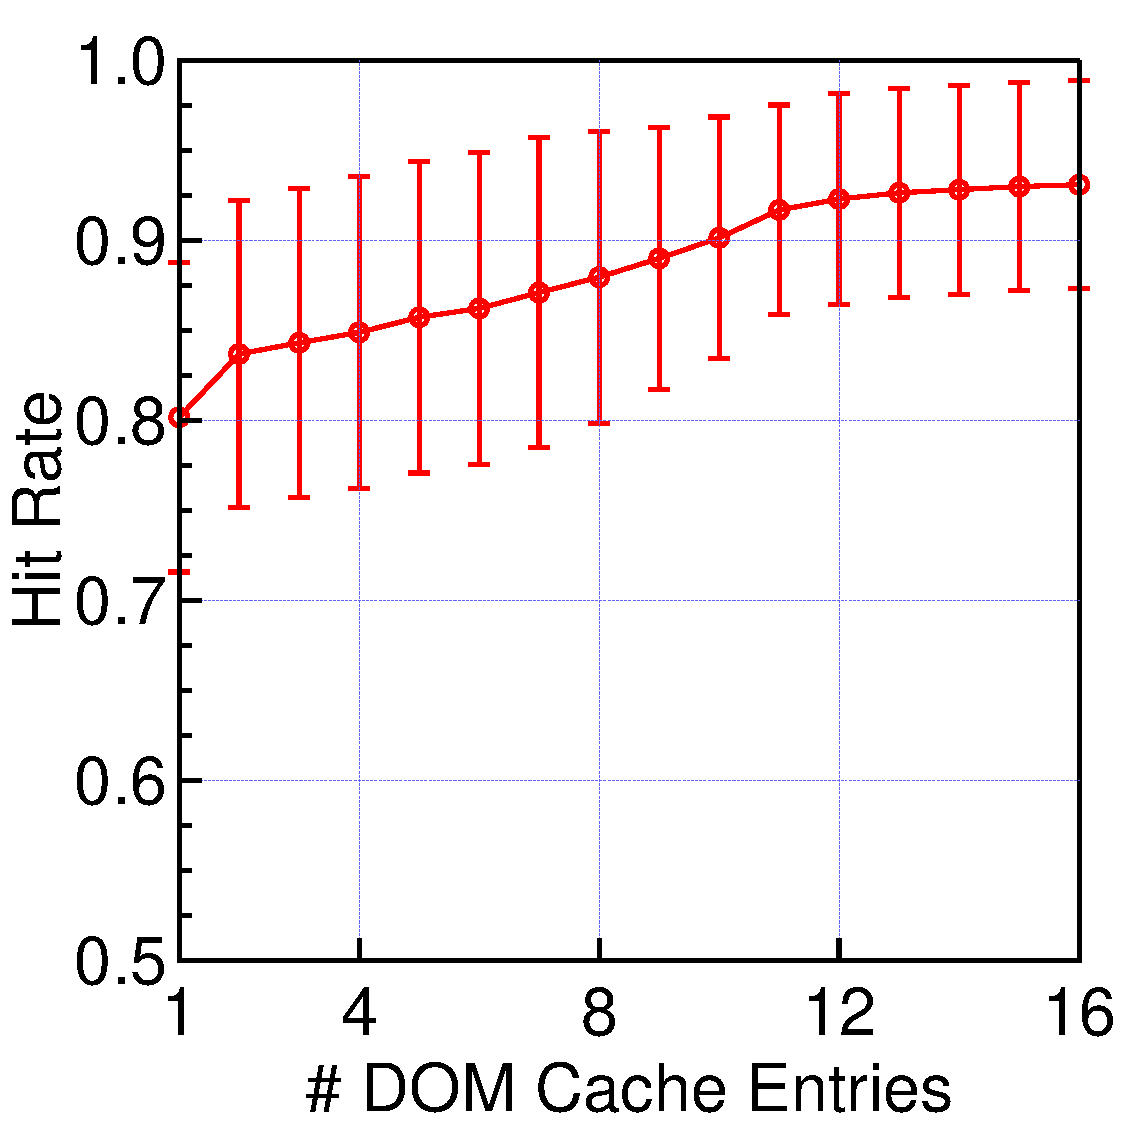
\includegraphics[trim=0 0 0 0, clip, width=.45\columnwidth]{hit-rate}
	\label{fig:hit-rate}
} 
\caption{\small DOM tree access behavior across webpages.}
\label{fig:dom-loc}
\end{figure}

The DOM tree and Render tree are the two most important data structures because they are shared across different kernels. We propose the Browser Engine Cache to improve the energy-efficiency of accessing them. Specifically, the browser engine cache consists of a DOM cache and a Render cache for the DOM tree and Render tree, respectively. We use the DOM to explain our locality observation. Similar analysis and design principles also apply to the render cache. Note that the browser engine cache focuses on improving the energy efficiency of data feeding. We will discuss techniques for improving the performance aspect of data accesses in \Sect{sec:arch:related}.

The energy inefficiency of the traditional cache is best embodied in the performance-oriented design P2 in~\Tbl{tab:dse:ednp}. P2 requires a larger data cache (64~KB) compared to a traditional mobile core. Although a large cache achieves a high hit rate of 93\%, it leads to almost one-fourth of the total energy consumption. However, through careful characterizations, we find that accesses to the DOM/Render tree have strong locality and regular access pattern such that they can benefit from a small and energy-efficient cache memory, rather than the large power-hungry traditional caches. Let us explain our observations below.

First, we find that data accesses to the DOM tree have heavy reuses. \Fig{fig:con-reuse} shows the cumulative distribution of DOM tree node reuse. Each~($x, y$) point corresponds to a portion of DOM tree nodes~($y$) that are consecutively reused at least a certain number of times~($x$). About 90\% of the DOM tree nodes are consecutively reused at least three times, which reflects strong data locality. This indicates that a very small cache can achieve the similar hit rate as a regular cache, but with much lower power.

Second, we find that the accesses to the DOM tree have regular stream-like patterns. To illustrate this,~\Fig{fig:data-acs} shows two representative data access patterns to the DOM tree from \website{www.sina.com} and \website{www.slashdot.org}. Each ($x, y$) point is read as follows. The $x$-th access to the DOM tree operated on the $y$-th DOM node. We observe a common streaming pattern. Such a streaming pattern is due to the intensive DOM tree traversal that is required by many rendering engine kernels. For example, in order to match CSS rules with descendant selectors such as~``\texttt{div p},'' which selects any~\texttt{$<$p$>$} element that is a descendant of~\texttt{$<$div$>$} in the DOM tree, the~\textit{Style} kernel must traverse the DOM tree, one node at a time, to identify the inheritance relation between two nodes. Similarly, the~\textit{Layout} kernel must traverse the Render tree (recursively) to determine the size of each webpage element, which in turn depends on the sizes of the elements contained within it.

In summary, the rendering engine typically operates on one DOM tree node heavily and traverses to the next one. After the rendering engine moves past a DOM node, it is rarely re-referenced soon. Such a unique access behavior motivates the browser engine cache design as we describe below.

\subsection{Hardware Design}
\label{sec:cache:hw}

We propose the DOM cache to capture the DOM tree data locality. It sits between the processor and the L1 cache, effectively behaving as an L0 cache. Each cache line contains the entire data for one DOM tree node, which is 698~bytes in our design. Different from the data array in a regular cache, we implement each cache entry (both in the DOM cache and render cache) as a collection of registers instead of a wide cache line.  Each register holds one attribute of the DOM (Render) tree node, and can be individually accessed through special memory instructions from the software.

The motivations to split each DOM cache line into individually addressable registers are as follows. First, not all the attributes of a node are accessed every time a node is referenced such that pre-loading all the node data from L1 cache to the browser engine cache lead to performance and energy penalty. For example, a Render tree node most often is of either \texttt{RenderBlock} or \texttt{RenderInline} type, each of which involves its own set of attributes. The browser can decide what attributes to load depending on what type a Render tree node is. Second, splitting the large memory array into small registers also allows fast and more energy-conserving accesses.

We choose to implement the DOM cache as a ``software-managed'' cache--i.e., the data is physically stored in hardware memory, and the software performs the actual cache management, such as insertion and replacement. Prior work has demonstrated effective software-managed cache implementations~\cite{Hallnor:2000:FAS:339647.339660}. It is possible to implement the DOM cache entirely in hardware, similar to a normal data cache. Our motivation for a software-managed cache is to avoid the complexity of a hardware cache. Typically, the cache involves hardware circuitry whose overhead can be high, especially for extremely small cache sizes.

\begin{figure}[t]
\centering
\subfloat[\small{\website{www.sina.com.cn}}]
{
	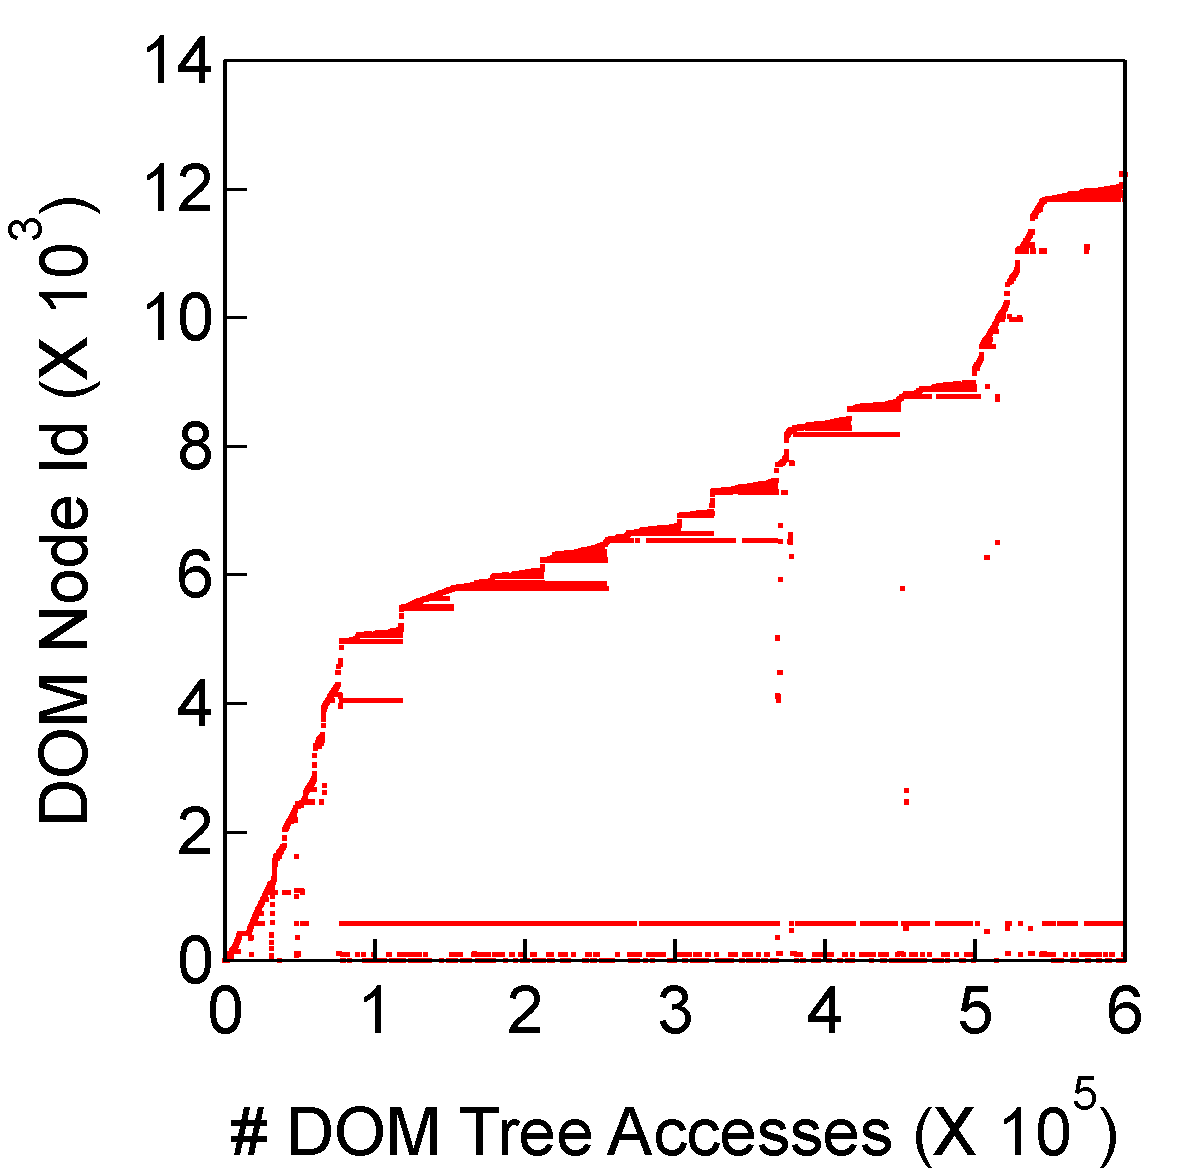
\includegraphics[trim=0 0 0 0, clip, width=.45\columnwidth]{sina}
	\label{fig:sina}
}
\hspace*{15pt}
\subfloat[\small{\website{www.slashdot.org}}]
{
	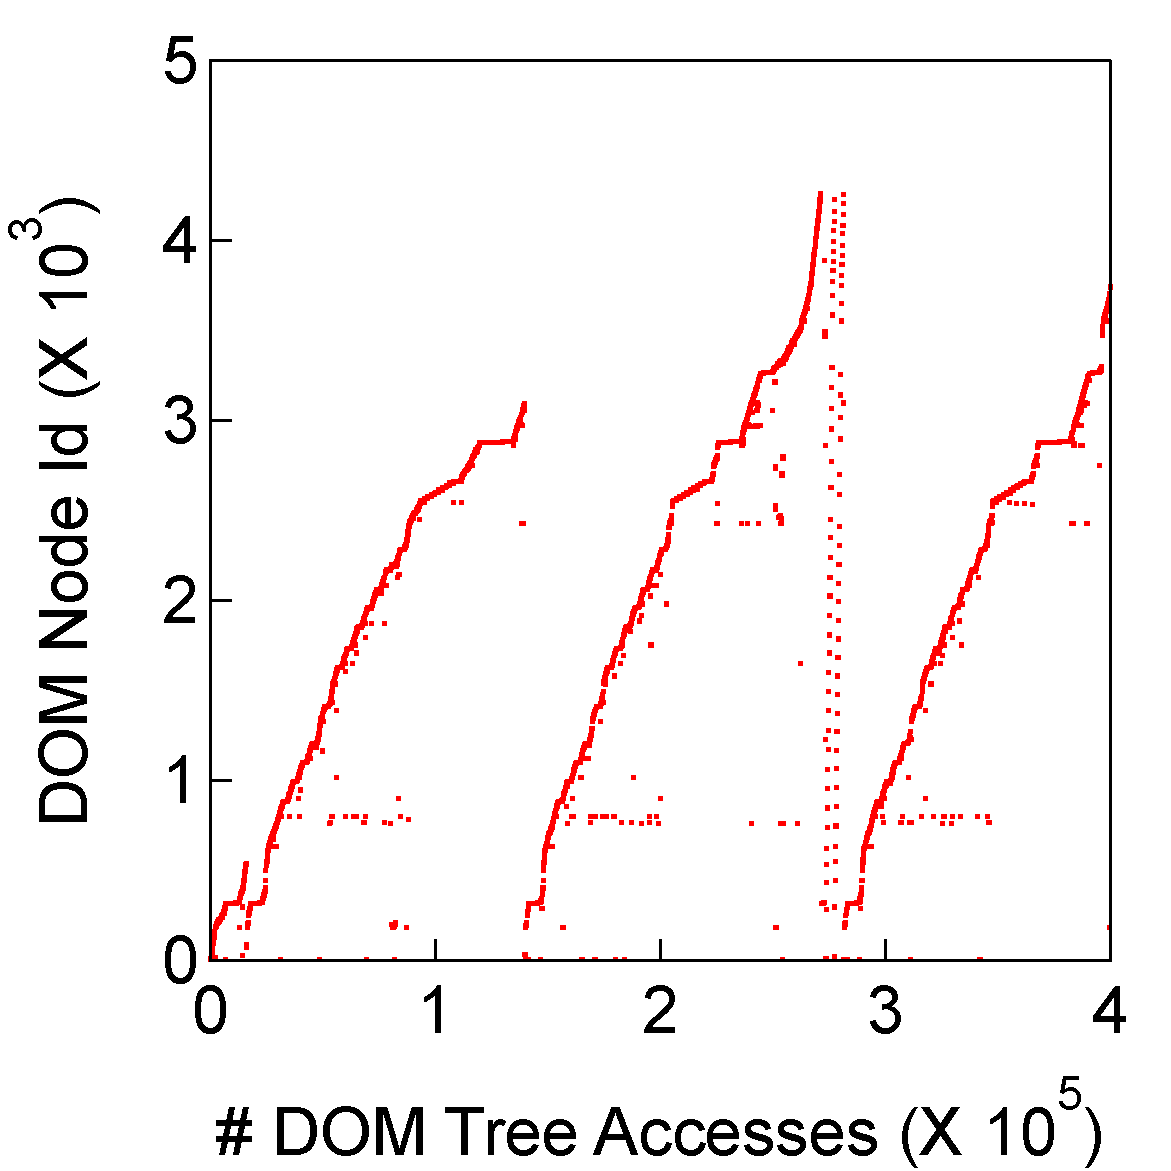
\includegraphics[trim=0 0 0 0, clip, width=.45\columnwidth]{slashdot}
	\label{fig:slashdot}
} 
\caption{\small Representative DOM tree access patterns.}
\label{fig:data-acs}
\end{figure}

The software overhead for the software-managed browser cache is relatively insignificant for the following reasons. First, a simple replacement policy that always evicts the earliest inserted line is sufficient. Due to the streaming pattern shown in~\Fig{fig:data-acs}, DOM tree nodes are rarely re-referenced soon after the browser engine moves past them. Therefore, a simple FIFO design is almost as effective as the least recently used policy, but with much less management overhead.

Second, a very small number of DOM cache entries guarantee a high hit rate. Therefore, the cache-hit lookup overhead is minimal.~\Fig{fig:hit-rate} shows how the hit rate changes with the number of entries allocated for the DOM tree. The curve represents the average hit rate, and the error bars represent the standard deviations across different webpages. Across all the webpages, a 4-entry design can achieve about 85\% hit rate, and so we use this configuration. In this sense, the DOM cache is effectively a single set, 4-way fully associative cache. Similarly, the render cache contains two entries (i.e., two cache lines). On average, it achieves over 90\% hit rate.

\subsection{Software Support and Programmability}
\label{sec:cache:sw}

To access a particular DOM tree node in the rendering engine, developers issue~\texttt{DOMCache\_LD(Id, attr)} and~\texttt{DOMCache\_ST(Id, attr, data)} for read and write operation, respectively. Similar APIs are also provided for the Render Cache. In the provided APIs, \texttt{Id} represents the DOM tree node ID (similar to the \texttt{Style\_Apply()} API), \texttt{attr} represents a particular DOM node attribute, and \texttt{data} indicates the new data of the specified \texttt{attr}. Recall that our DOM cache design allows each attribute of a DOM node to be individually addressed~(\Sect{sec:cache:hw}). The syntax of both APIs allow developers to fully utilize this feature.

\begin{figure}[b]
\centering
\captionsetup{width=\columnwidth}
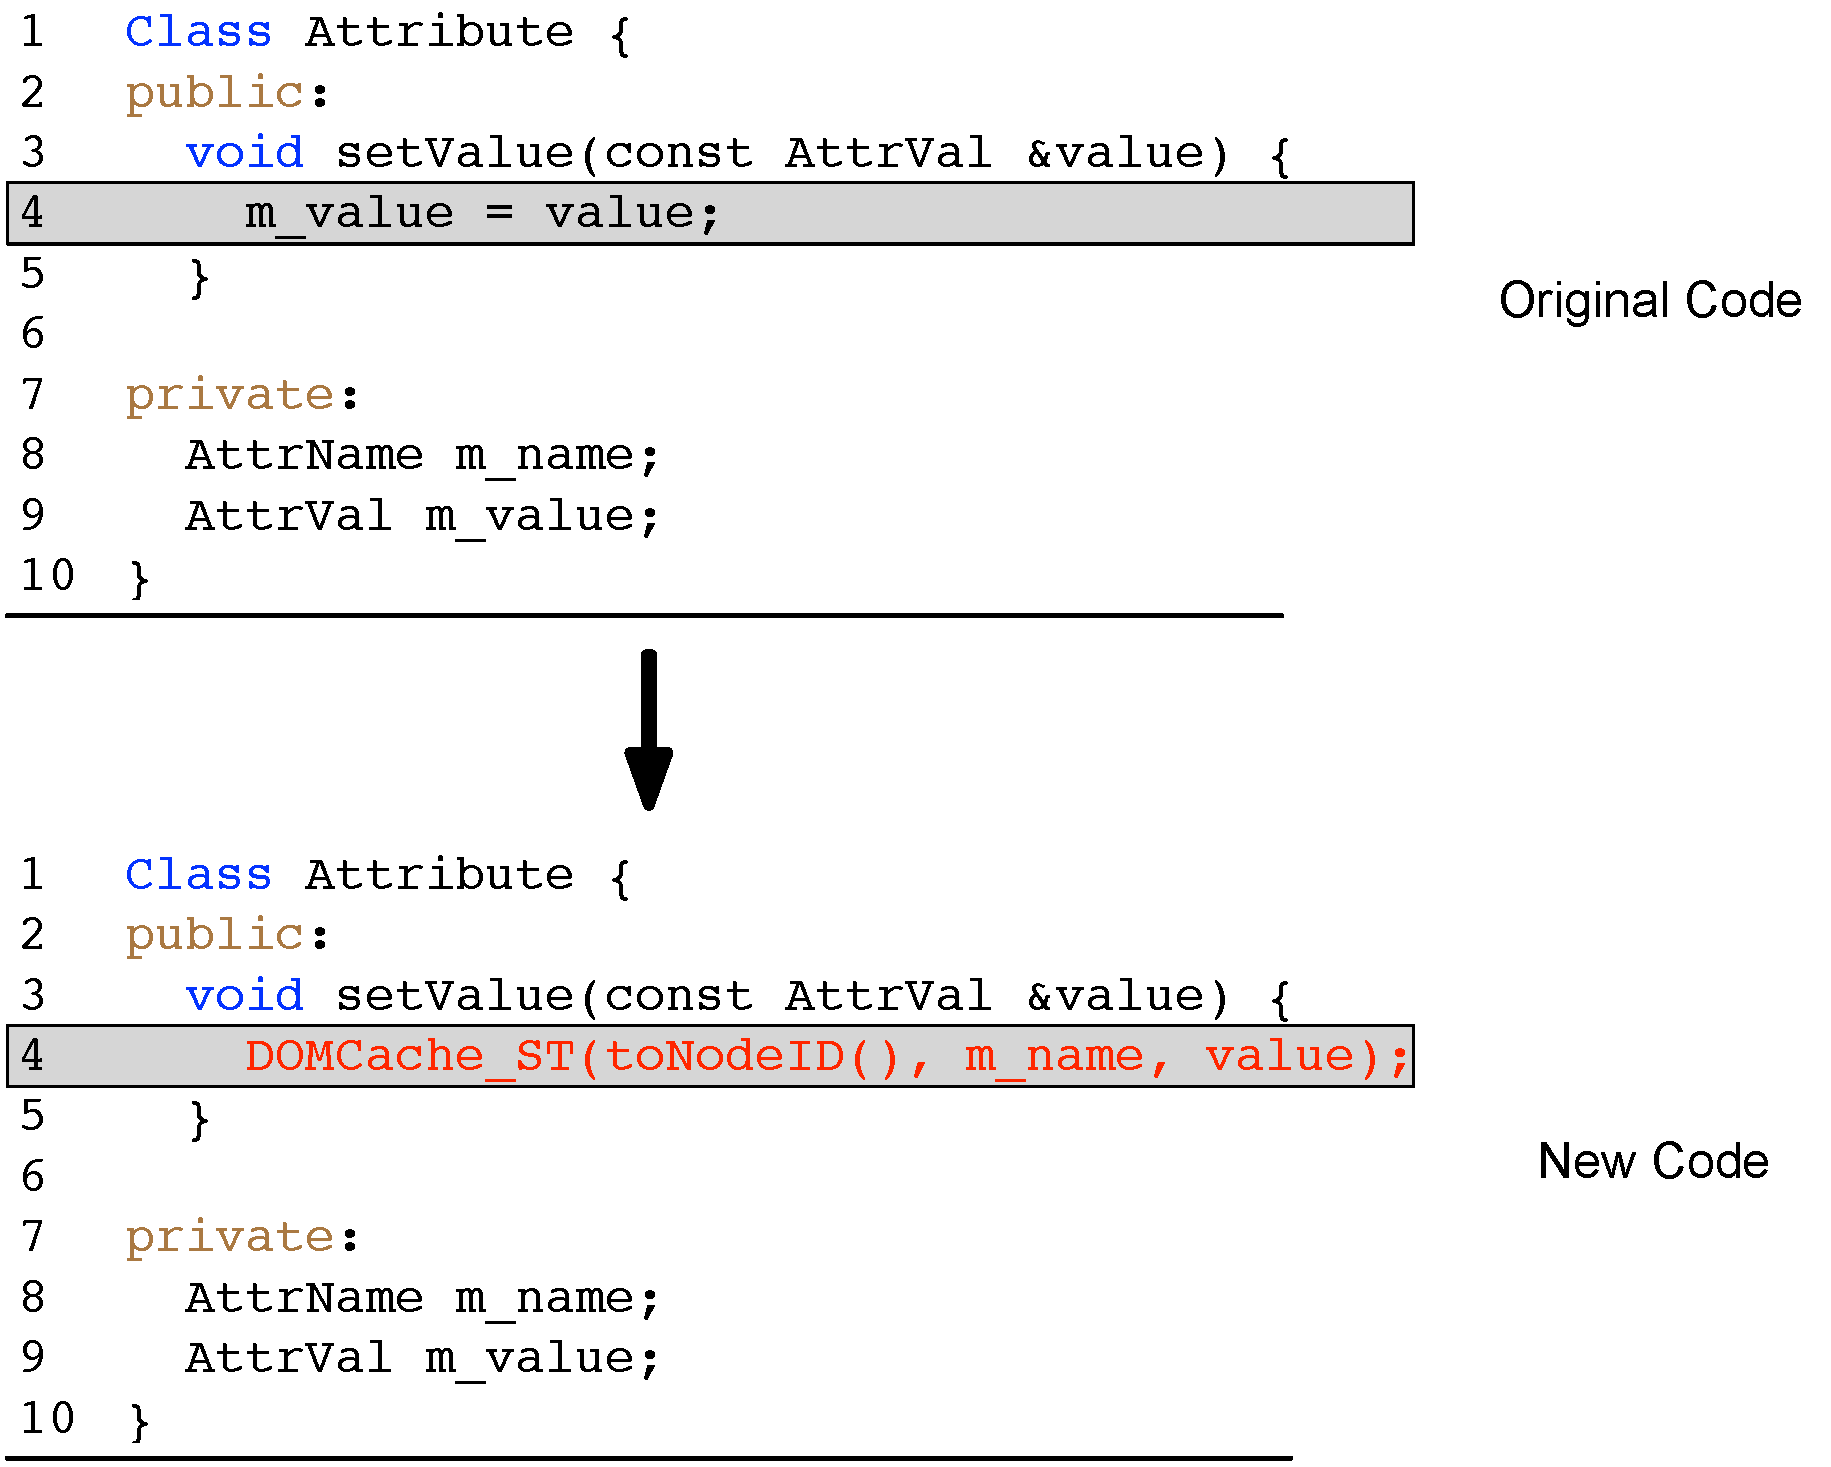
\includegraphics[trim=0 0 0 0, clip, width=\columnwidth]{style-code-cache}
\caption{\small{Using the \texttt{DOMCache\_ST()} API in the rendering engine. The new DOM attribute store API replaces the original attribute value assignment, and performs cache manegement.}}
\label{fig:style-code-cache}
\end{figure}

\Fig{fig:style-code-cache} shows how \texttt{DOMCache\_ST()} API is used in the rendering engine. It is used to set value of any given attribute in the \texttt{setValue()} method of the \texttt{Attribute} class. Specifically, \texttt{DOMCache\_ST()} replaces the original value assignment. The API implementation performs the actual hardware memory accesses as well as cache management, such as replacement and insertion. For example, the API needs to maintain an array, similar to the tag array in a regular cache, to keep track of which DOM nodes are in the cache and whether they are modified.  Effectively, the runtime library of DOM cache APIs implements a cache simulator. However, the runtime overhead is negligible due to the simple cache design as described in~\Sect{sec:cache:hw}.

It is worth noting that using DOM cache APIs only affects the primitive classes of a rendering engine (such as the \texttt{Attribute} class in \Fig{fig:style-code-cache}) while maintaining the interface between primitive classes and the rest of the rendering engine unchanged. For example, rendering engine developers can still use the same \texttt{setValue()} method to update an attribute's value. Therefore, we do not expect using the new APIs to affect the development productivity.

\section{WebCore Evaluation}
\label{sec:arch:eval}

In this section, we first present the power and timing overhead analysis of the proposed specialization techniques~(\Sect{sec:arch:eval:oh}). We then evaluate the energy-efficiency implications of the SRU and the browser engine cache individually~(\Sect{sec:arch:eval:sru}, \Sect{sec:arch:eval:cache}). In the end, we show the energy-efficiency improvement combining both customization and specialization~(\Sect{sec:arch:eval:comb}). In particular, we show that our specializations can achieve significantly better energy efficiency than simply dedicating the same amount of area and power overhead to tune the conventional general-purpose cores.

We evaluate our optimizations against three designs, D1 through D3. D1 refers to the energy-conscious design (P1) that we explored in~\Fig{fig:ivso}. Similarly, D2 refers to the performance-oriented design (P2) in~\Fig{fig:ivso}. D3 mimics the common design configuration of current out-of-order mobile processors. We configure D3 as a three-issue out-of-order core with 32-entry load queue and store queue, 40 ROB entries, and 140 physical registers. It has a 32~KB, 1-cycle latency L1 data and instruction cache, and a 1~MB, 16-cycle latency L2 cache.

\subsection{Overhead Analysis}
\label{sec:arch:eval:oh}

We use CACTI v5.3~\cite{cacti} to estimate the memory structures overhead. We implement the SRU in Verilog and synthesize our design in 28~nm technology using the Synposys toolchain.

\paragraph{Area} The size of SRU's scratchpad memory is 1~KB. The DOM cache size is 2,792~bytes. The render cache size is 1,036~bytes. The hardware requirements for the SRU are mainly comparators and MUXes to deal with control flow, and simple adders with constants inputs to compute each CSS property's final value. In total, the area overhead of the memory structures and the SRU logic is about 0.59~mm\textsuperscript{2}, which is negligible compared to typical mobile SoC size (e.g., Samsung's Exynos 5410 SoC has a total die area size of 122~mm\textsuperscript{2}~\cite{exynox5410diesize}).

\paragraph{Power} The synthesis reports that the SRU logic introduces 70~mW total power under typical stimuli. The browser engine cache and the SRU scratchpad memory add 7.2~mW and 2.4~mW to the dynamic power, respectively. They are insignificant compared to power consumption for Web browsing (in our measurements, a single core Cortex-A15 consumes about 1~W for webpage loading). Clocking gating can reduce the power consumption further~\cite{queuethermal}. But we are conservative in our analysis and do not assume such optimistic benefits.

\paragraph{Timing} Both the browser engine cache and SRU scratchpad memory can be accessed in one cycle, which is the same as the fastest L1 cache latency in our design space. The synthesis tool reports that the SRU logic latency is about 16 cycles under 1.6~GHz. Later in our performance evaluation, we conservatively assume the SRU logic is not pipelined.

\paragraph{Software} The software overhead mainly includes cache management and SRU compensation code creation. The overhead varies depending on individual webpage runtime behaviors. We model these overheads in our performance evaluation and discuss their impact along with the improvements.

\subsection{Style Resolution Unit}
\label{sec:arch:eval:sru}

\begin{figure}[t]
\centering
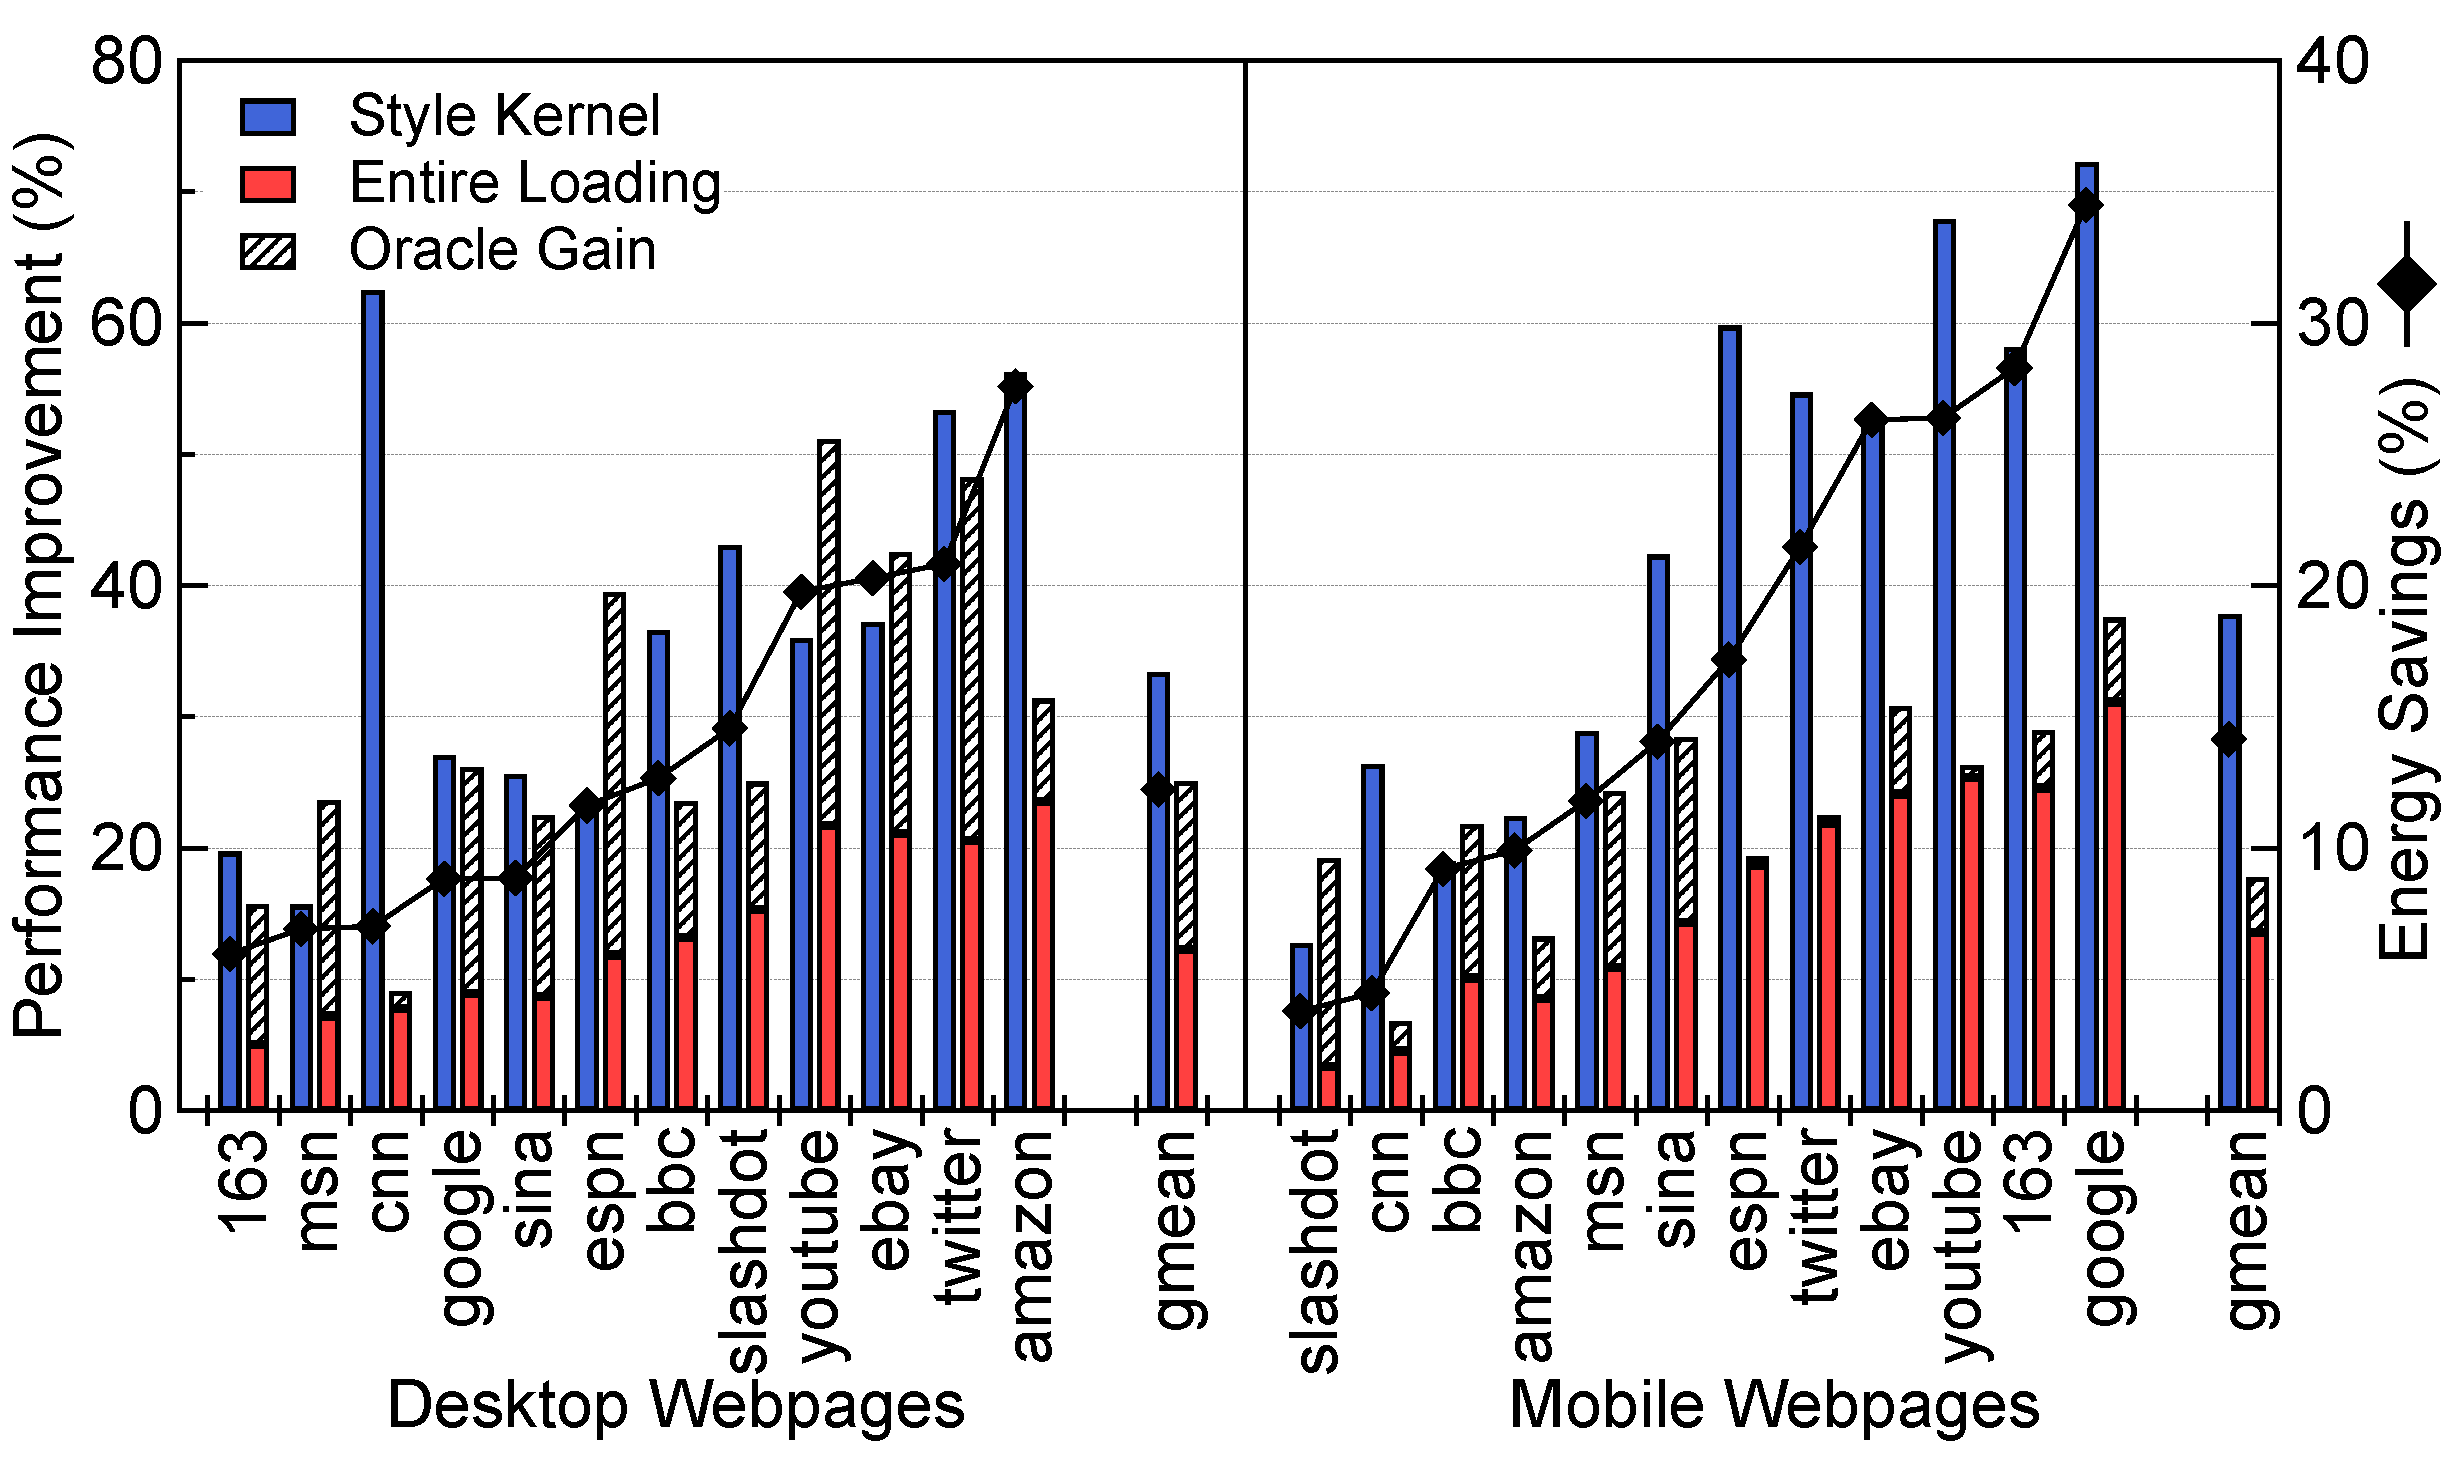
\includegraphics[trim=0 0 0 0, clip, width=\columnwidth]{sru-perf}
\caption{\small{Performance and energy improvement of the SRU.}}
\label{fig:sru-perf}
\end{figure}

Our SRU prototype design achieves on average 3.5X, and up to 10X, speedup for the accelerated style applying phase. The improvements vary because of individual webpage characteristics.

\Fig{fig:sru-perf} shows SRU's performance improvement for the~\textit{Style} kernel and the entire webpage loading on the performance-oriented design D2 in \Fig{fig:ivso}.  The average performance improvement of the~\textit{Style} kernel is 33.4\% and 37.8\% for desktop and mobile webpages, respectively. Generally, we find that mobile webpages benefit slightly more from the SRU because they tend to be less diversified in webpage styling, and therefore the SRU has higher coverage.

The overall improvements vary across webpages because different webpages spend different portions of time in the~\textit{Style} kernel. For example, \website{cnn} spends only 14\% of its execution time in the~\textit{Style} kernel during the entire run. Therefore, its 62\% improvement in the~\textit{Style} kernel translates to an overall improvement of only 7\%. On average, the SRU improves the entire webpage load time by 13.1\% on all the webpages.

The SRU not only improves performance but also reduces energy consumption. The right $y$-axis of~\Fig{fig:sru-perf} shows the energy saving for the entire webpage loading. Webpages are sorted according to the energy savings. On average, SRU results in 13.4\% energy saving for all webpages.

\Fig{fig:sru-perf} also shows the oracle improvement if the entire applying phase can be delegated to the SRU (i.e., no hardware resource constraints). Desktop webpages have much higher oracle gain than mobile webpages. The software fall-back mechanism is more frequently triggered in desktop-version webpages due to their diversity in styling webpages. This also implies the potential benefits of reconfiguring the SRU according to different webpages. An SRU that is customized for mobile webpages could potentially be much smaller.

We apply the SRU to different designs to show its general applicability. For loading an entire webpage, on a current mobile processor design (D3), the SRU improves performance by 10.0\% and reduces energy consumption by 10.3\%. On an energy-conscious design (D1), it improves performance by 8.4\% and reduces energy consumption by 11.6\%.

\subsection{Browser Engine Cache}
\label{sec:arch:eval:cache}

\Fig{fig:cache-energy} shows the energy reduction from using the browser engine cache. The browser engine cache can serve data more energy-efficiently because of the high hit rate of its cache (as shown in~\Fig{fig:hit-rate}). Mobile webpages achieve less energy saving than desktop-version webpages because of their smaller memory footprint. On average, the performance-oriented design (D2) achieves 14.4\% energy savings. Since the energy-conscious (D1) and current design (D3) have smaller caches, the energy consumption caused by the data cache is less, and therefore benefits less from the browser engine cache. On average, their energy consumption reduces by 5.9\% and 9.3\%, respectively.

\begin{figure}[t]
\centering
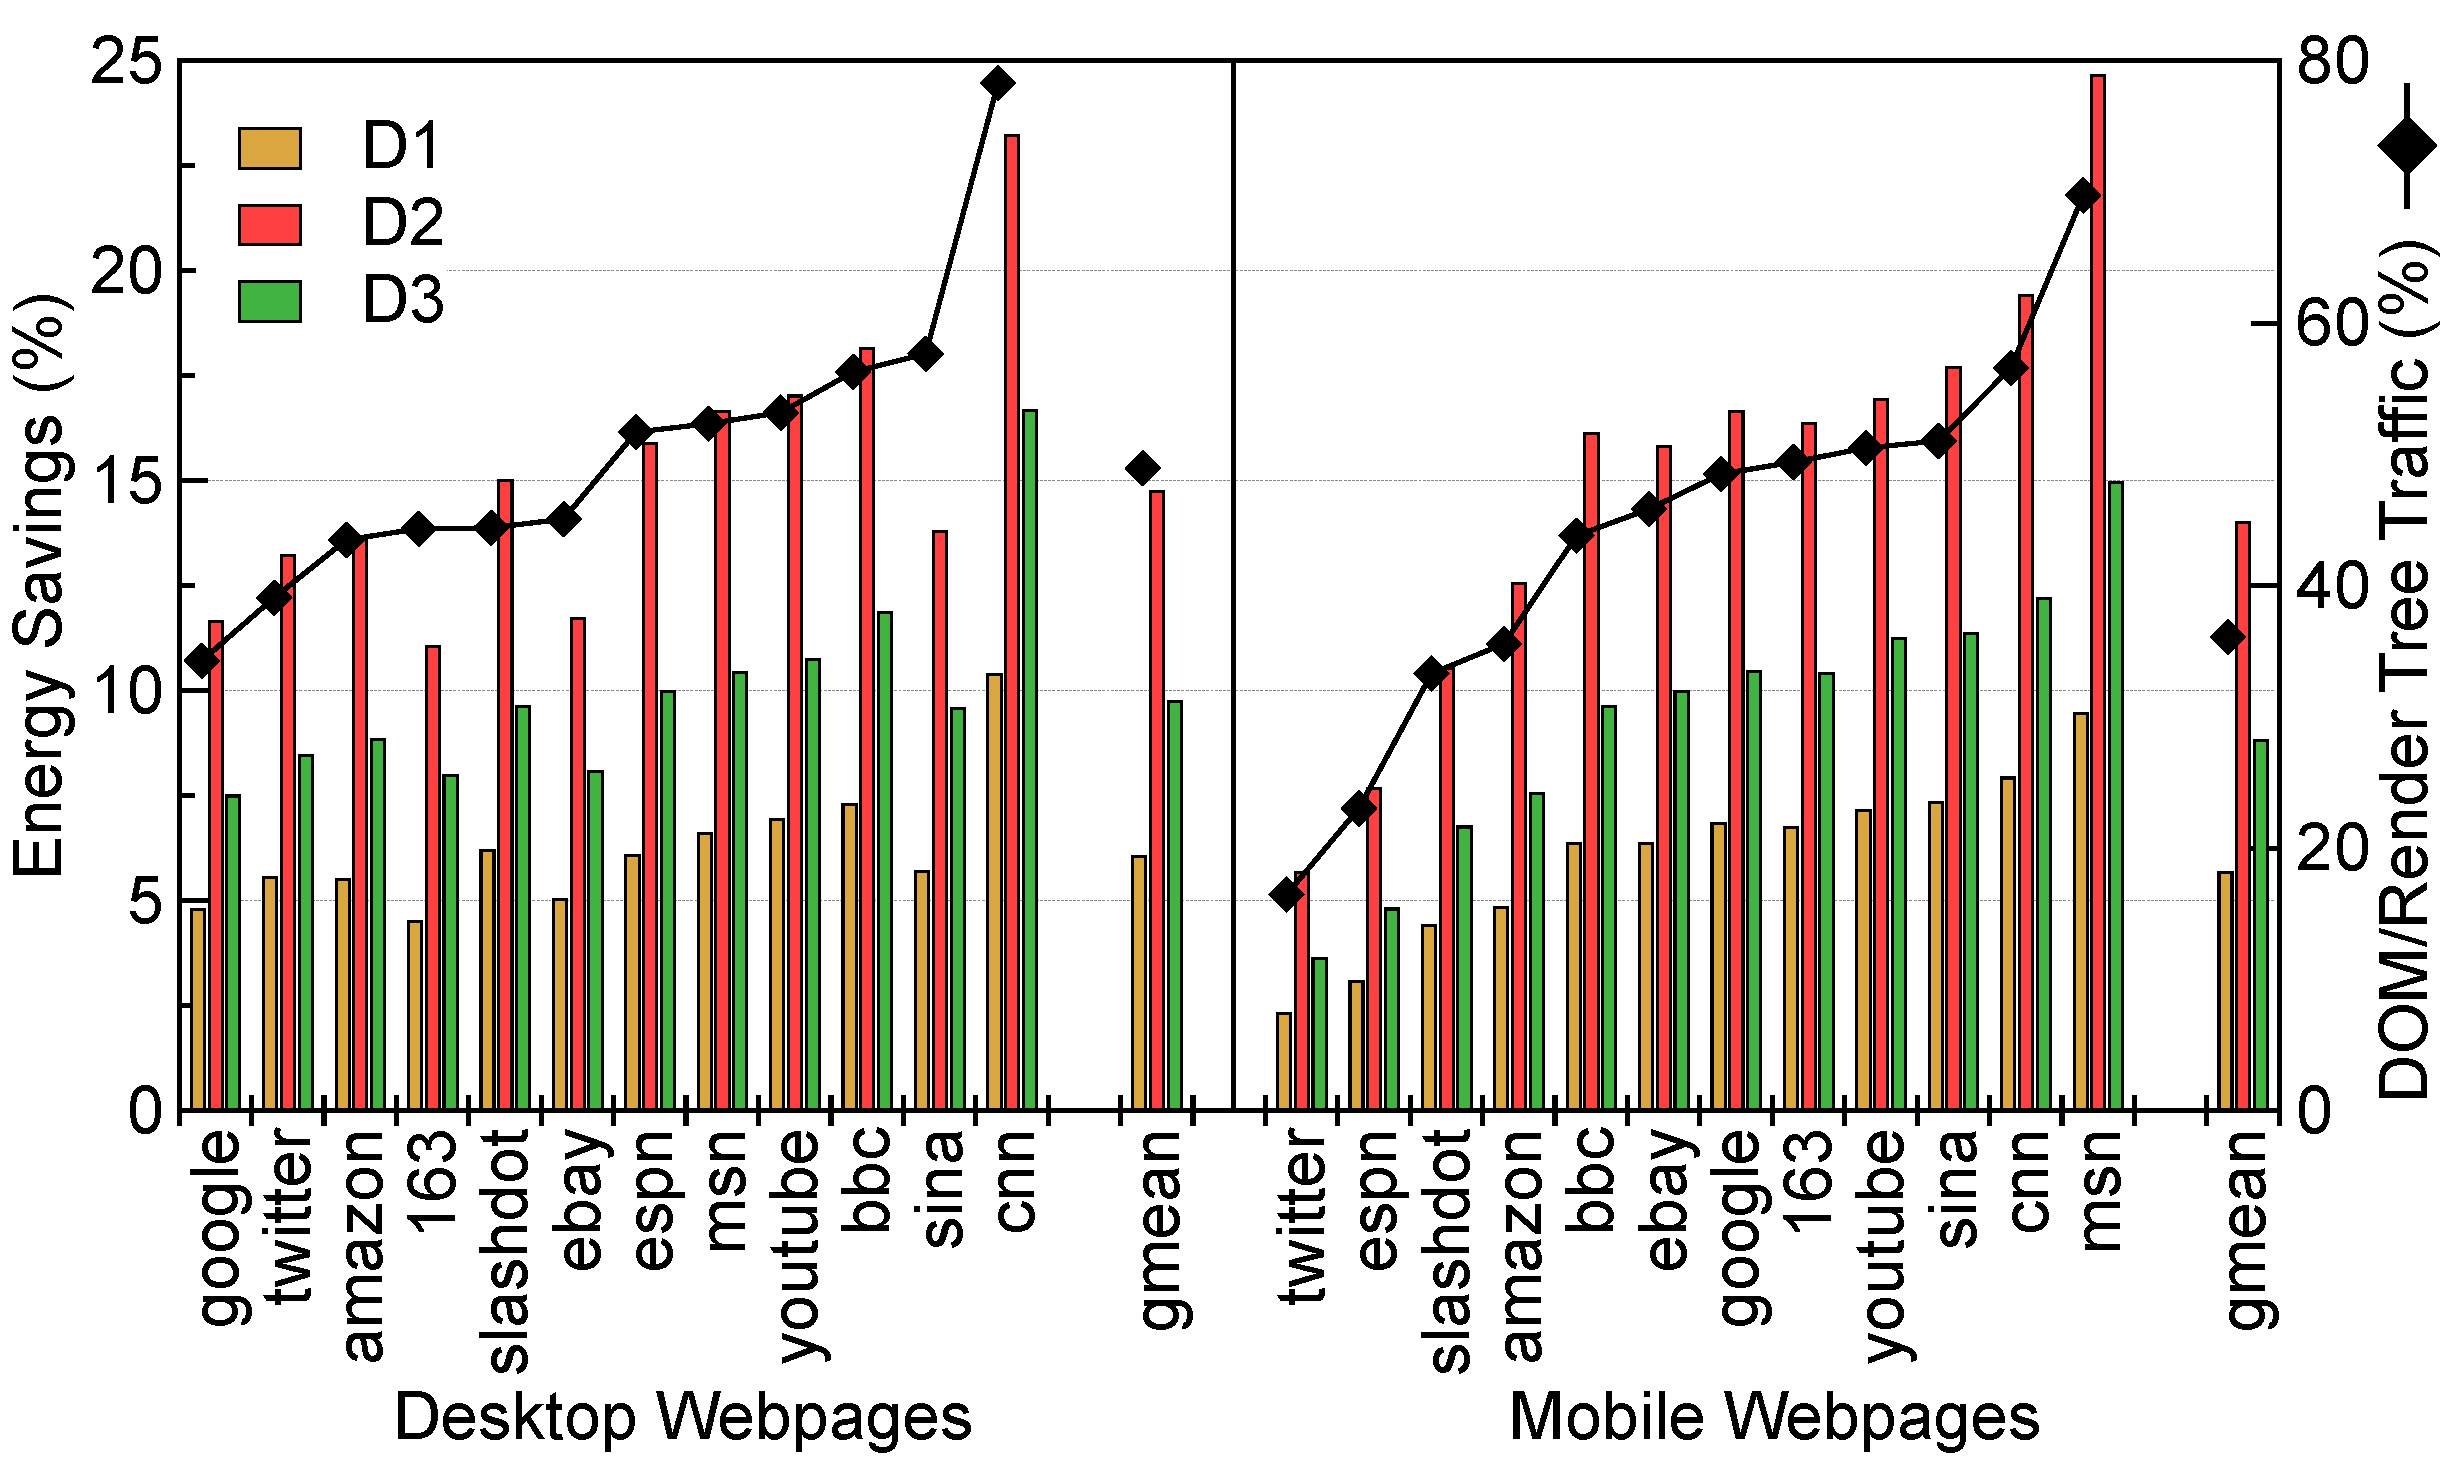
\includegraphics[trim=0 0 0 0, clip, width=\columnwidth]{cache-energy}
\caption{\small{Energy savings with a browser engine cache.}}
\label{fig:cache-energy}
\end{figure}

\begin{figure}[t]
\centering
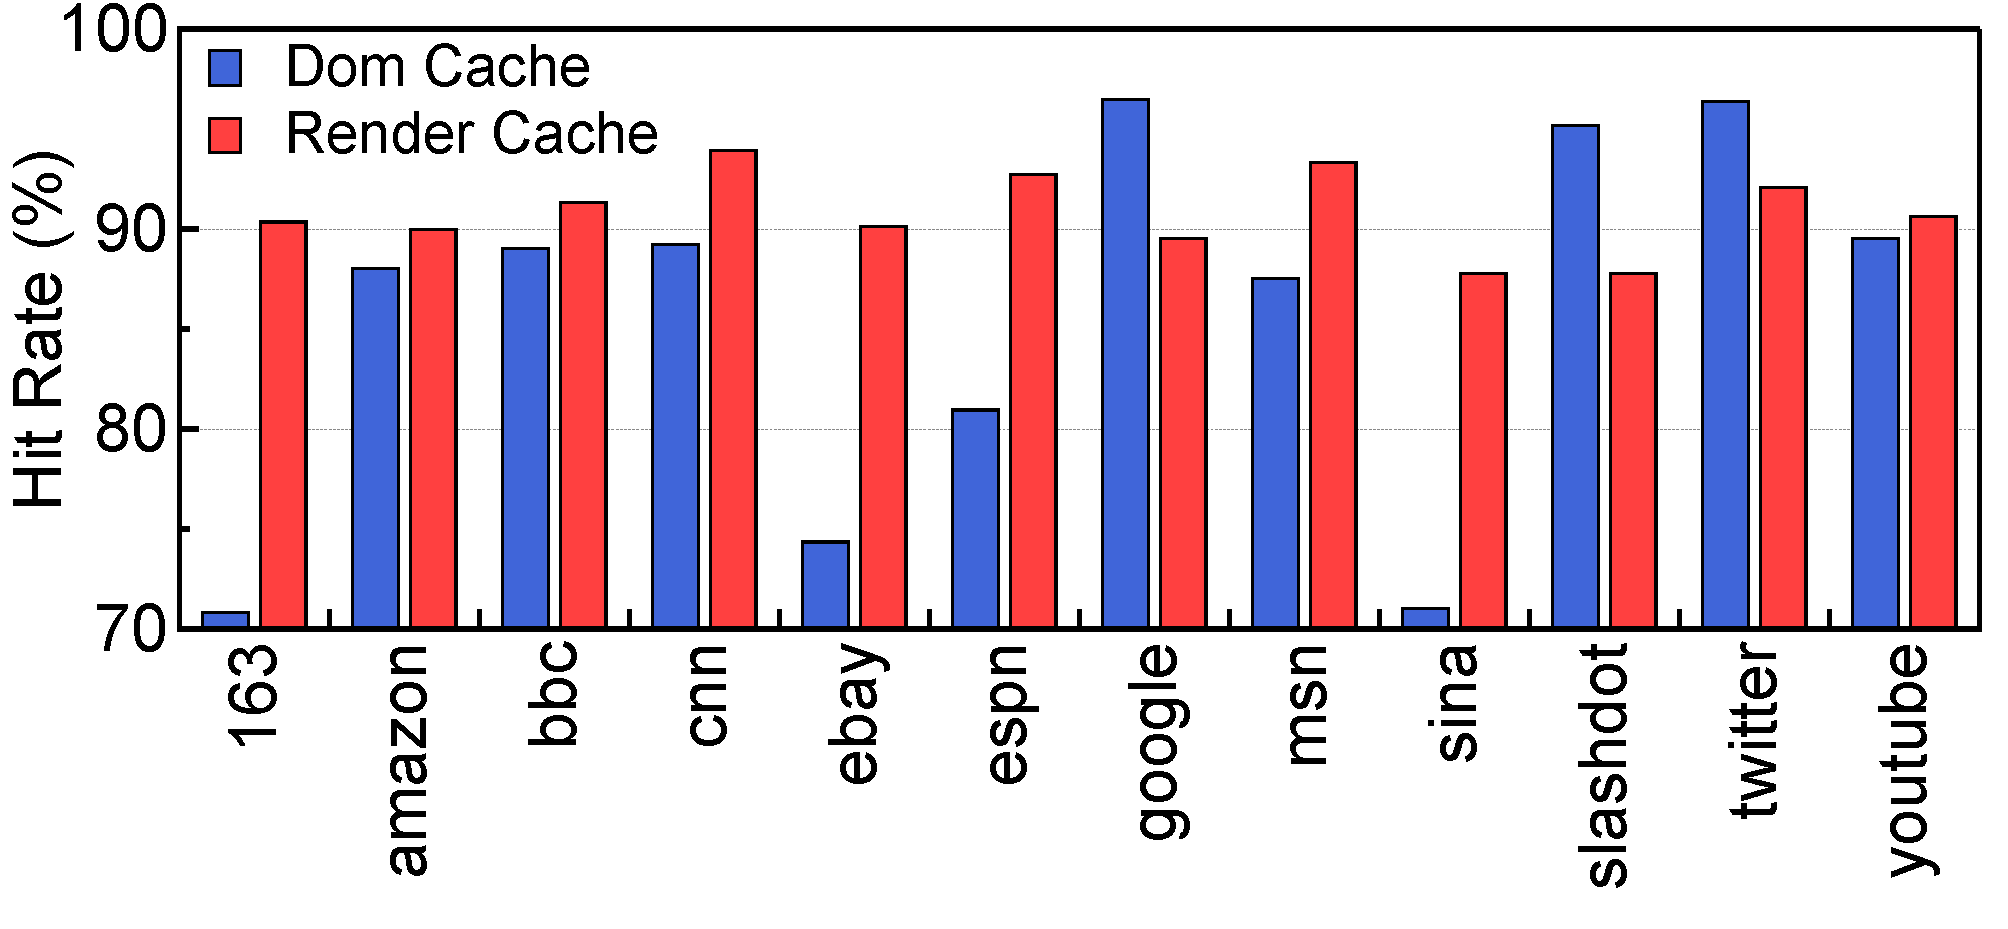
\includegraphics[trim=0 0 0 0, clip, width=.9\columnwidth]{hit-rate-page}
\caption{\small{DOM Cache and Render Cache hit rate for desktop webpages.}}
\label{fig:hit-rate-page}
\end{figure}

\begin{figure}[t]
\centering
\captionsetup{width=.9\columnwidth}
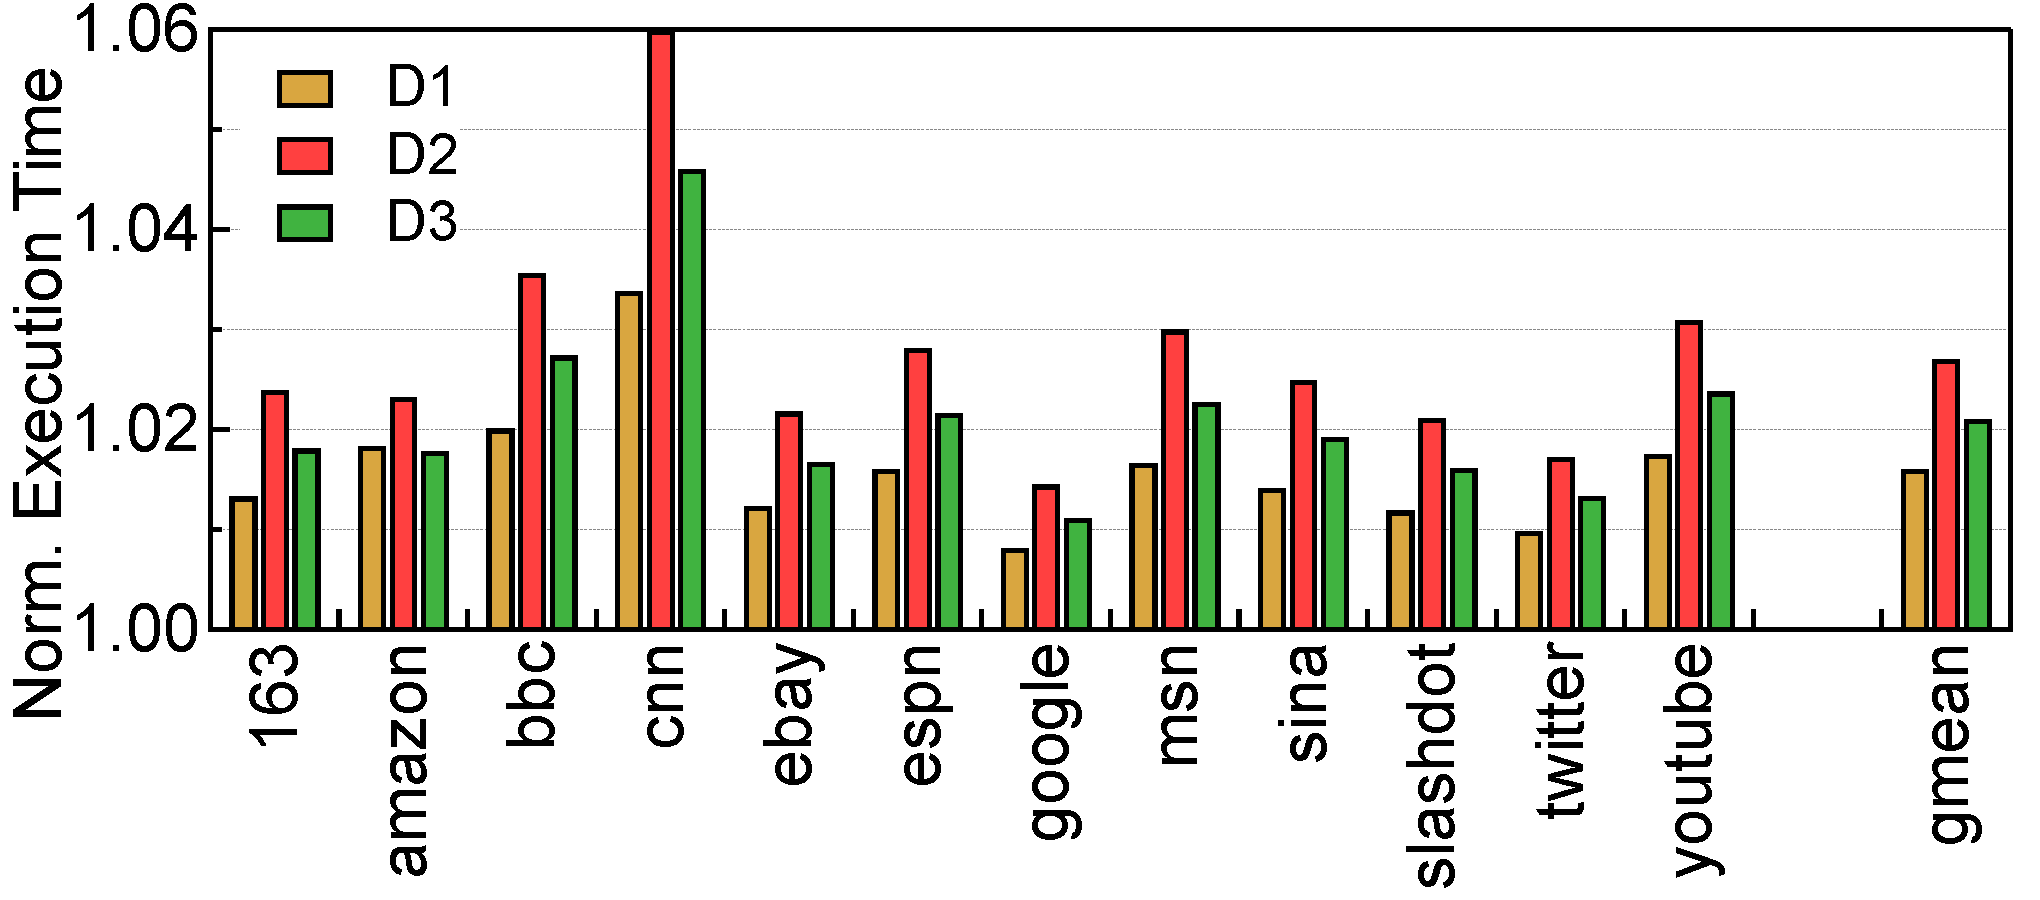
\includegraphics[trim=0 0 0 0, clip, width=.9\columnwidth]{cache-perf}
\caption{\small{Execution time with the browser engine cache of the three designs. Values are normalized to each design's baseline configuration without the browser engine cache.}}
\label{fig:cache-perf}
\end{figure}

We find that the DOM tree and Render tree access intensity largely determines the amount of energy saving. The right $y$-axis in~\Fig{fig:cache-energy} shows the amount of L1 data cache traffic that is attributed to accessing both data structures. In the most extreme case, about 80\% of the data accesses for loading~\website{cnn} touch the DOM tree and the Render tree. Therefore, it achieves the largest energy saving.

There are some outliers in desktop webpages where the energy savings are not proportional to DOM/Render tree access intensity. For example,~\website{sina} has a much higher traffic ($\sim$60\%) than~\website{twitter} ($\sim$40\%), but with similar energy savings. This is because~\website{sina} has a much lower DOM cache hit rate than~\website{twitter}. \Fig{fig:hit-rate-page} shows the DOM cache and Render cache hit ratio for desktop webpages. We observe that \website{sina} has a DOM cache hit rate at $\sim$70\%, lower than~\website{twitter} at $\sim$97\%. A lower DOM cache hit ratio indicates the \website{sina} does not fully use the low-energy browser engine cache. In contrast, we find that mobile webpages all have a high browser engine cache hit rate, and therefore their energy savings closely track the DOM/Render tree traffic.

Due to the software cache management overhead, the browser engine cache incurs performance overhead. \Fig{fig:cache-perf} shows the desktop webpages' execution time of the three designs with the browser engine cache. The values are normalized to each design's baseline configuration without the browser engine cache. We find that the performance slow down is minimal, primarily because the design decisions that we made (as described in~\Sect{sec:cache:hw}) minimize the software management overhead. On average, the slowdown for D2 with a 64~KB L1 data cache is only 2.7\%. The slowdown for D1 and D3 with smaller L1 data caches (8~KB and 32~KB, respectively) is slightly smaller--only 1.6\% and 2.1\%, respectively. We speculate that the reason is that both D1 and D3 have slower performance than D2, and as such, they amortize the overhead of the software cache management.

\subsection{Combined Evaluation}
\label{sec:arch:eval:comb}

\begin{figure}[t]
\centering
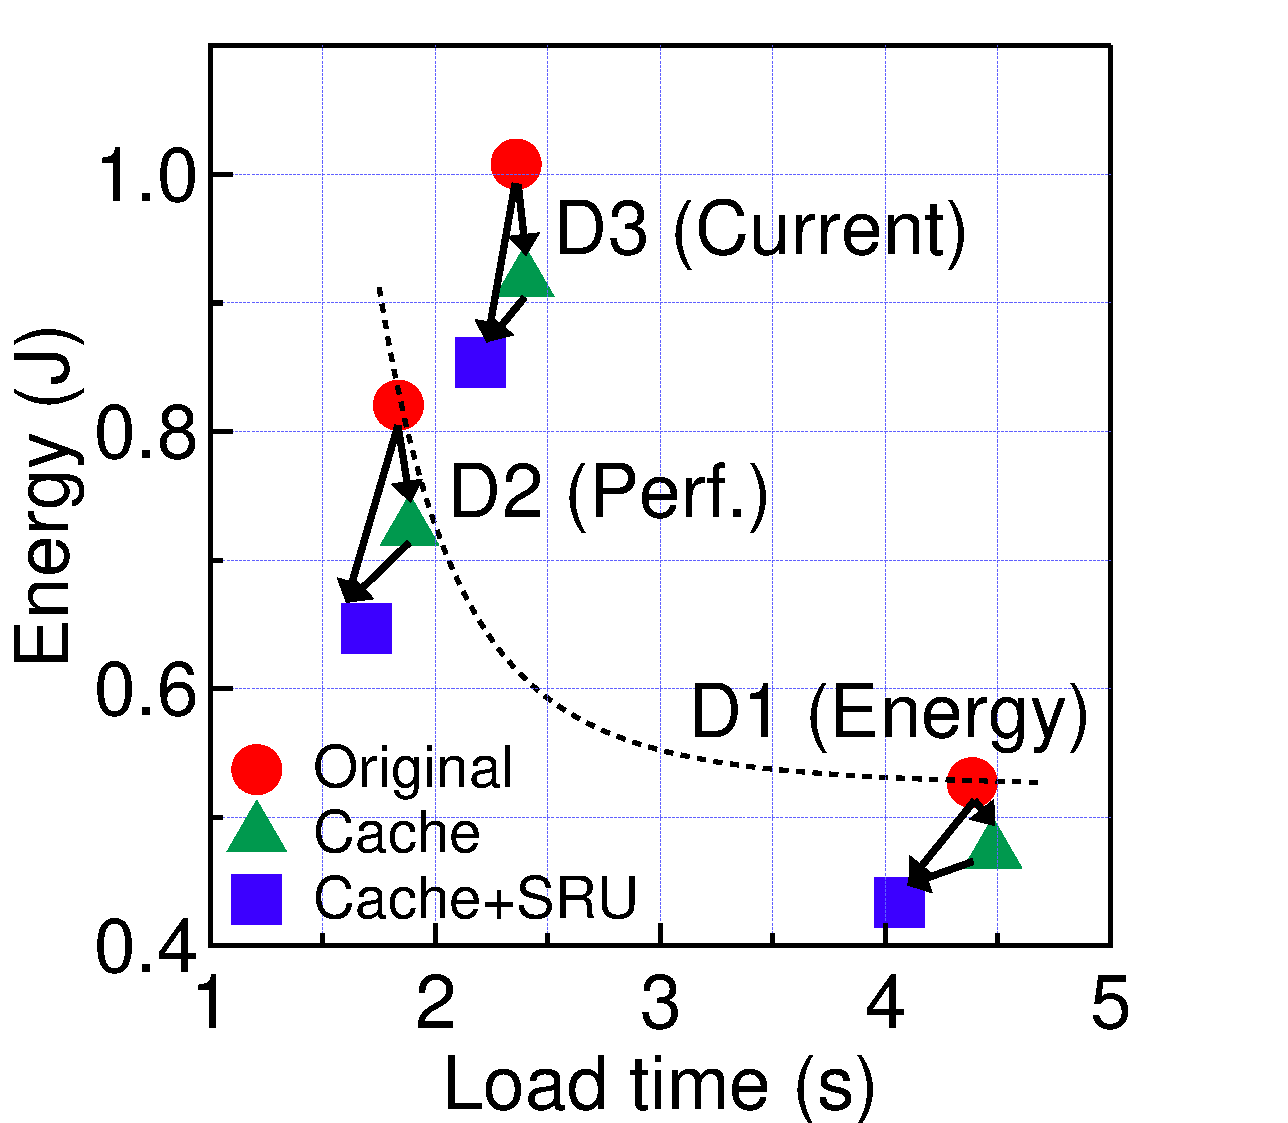
\includegraphics[trim=0 0 0 0, clip, width=.6\columnwidth]{dse-push}
\caption{Energy-efficiency improvement over three designs.}
\label{fig:dse-push}
\end{figure}

\Fig{fig:dse-push} shows the energy-efficiency improvement for the entire webpage loading on all three designs by progressively adding the two optimization techniques. The dotted curve represents the Pareto-optimal frontier of the design space discovered in~\Sect{sec:arch:customization:core}. The circles represent original designs in this energy-performance space. The triangles represent the new energy-performance trade-off points after applying the software-managed browser engine cache optimization. The squares show the new energy-performance points when the SRU is added atop the caching optimization.

Comparing the energy-conscious design (D2) with an existing mobile processor design (D3), we observe that customization of the general-purpose architecture alone without applying any specialization allows us to achieve 22.2\% performance improvement and 18.6\% energy saving.

After applying the browser engine cache, the performance slightly degrades due to its software management overhead. Therefore, all the triangles move slightly to the right despite the energy savings. However, applying the SRU optimization improves both performance and energy consumption. All the squares move toward the left corner. In effect, we push the Pareto-optimal frontier in the original design space to a new design frontier with significantly better energy efficiency.

In addition, we also observe that D3 with our specializations can now approach the original Pareto-optimal frontier. This implies that it is possible to apply specializations to existing mobile processors to achieve a similar level of energy efficiency as processors that are optimized for the mobile Web browsing workloads.

On average, the energy-conscious design (D1) benefits by 6.9\% and 16.6\% for performance improvement and energy reduction, respectively. The performance-oriented design (D2) benefits by 9.2\% and 22.2\% for performance improvement and energy reduction, respectively. Lastly, the existing mobile processor design (D3) benefits by 8.1\% and 18.4\% for performance improvement and energy reduction, respectively.

\begin{figure}[t]
\centering
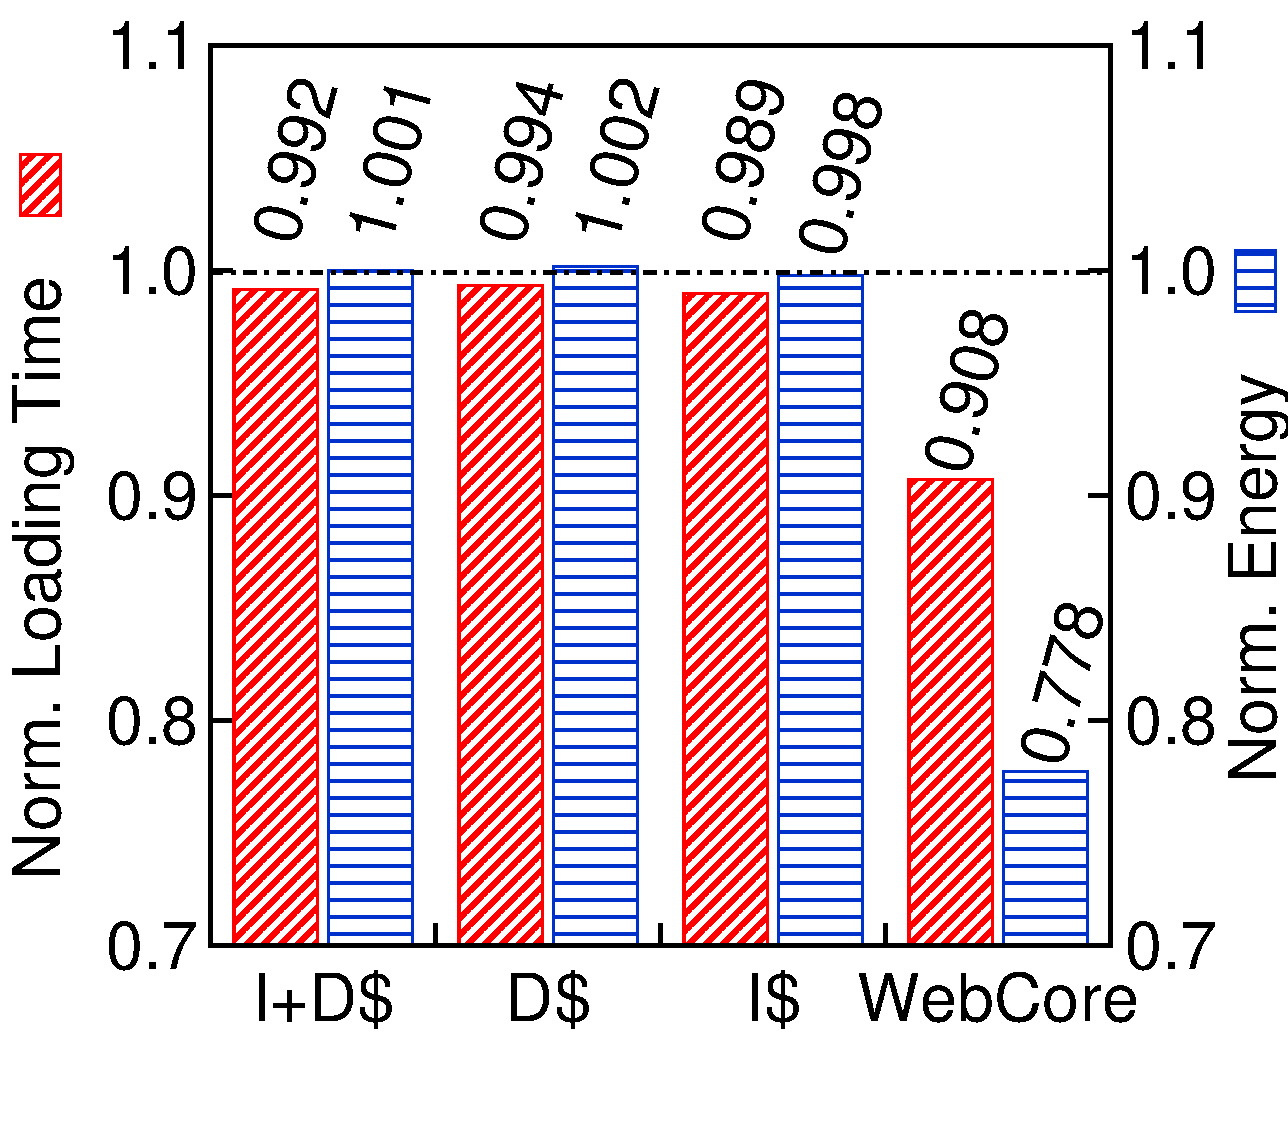
\includegraphics[trim=0 0 0 0, clip, width=.6\columnwidth]{compare-other}
\caption{Allocating area for caches versus specializations.}
\label{fig:compare-other}
\end{figure}

Our specializations incur area overhead. To quantitatively assess the effectiveness of the area overhead, we compare our results with general-purpose designs that simply use the same area overhead to scale up microarchitecture resources. In our evaluation, we use the additional area to improve the I-cache and D-cache sizes because instruction delivery and data feeding are the two major bottlenecks, as discussed in~\Sect{sec:arch:customization:sources}. The additional area would be most  justified to improve the I-cache and D-cache sizes.

As an example,~\Fig{fig:compare-other} compares our combined specializations (WebCore) with designs that increase the I-cache size by 24~KB (I\$), D-cache size by 24~KB (I\$), and both caches by 12~KB (I+D\$) based on the D2 design. The figure normalizes the webpage loading time and energy consumption to the D2 design without any specializations. We see that simply improving the cache sizes in general-purpose cores achieves only negligible performance improvement (\textless 1\%) with a slightly higher energy consumption. However, WebCore specializations provide significantly better energy efficiency.

\section{Related Work}
\label{sec:arch:related}

We first put \webcore in the broad context of architecture specialization for Web applications in \Sect{sec:arch:related:specialization}. The browser engine cache bears similarities with previous work on specialized cache design, which we discuss in \Sect{sec:arch:related:data}. Finally, \Sect{sec:arch:related:char} discusses prior work on constructing representative mobile Web benchmarks, which is inherently related to our Web application selection process.

\subsection{Architecture Specializations for the Web}
\label{sec:arch:related:specialization}

Similar to \webcore, SiChrome~\cite{SiChrome} performs aggressive specializations that map much of the Chrome browser into silicon. The key difference is that \webcore starts from a (well-optimized) general-purpose baseline and thus retains general-purpose programmability while still being energy-efficient. In addition, SiChrome evaluates energy-efficiency using the EDP metric while our Pareto optimal analysis provides a more generic optimization view than EDP.

EFetch~\cite{efetch} and ESP~\cite{esp} also propose specialized hardware structures on top of general-purpose cores to improve the performance and energy-efficiency of Web applications. They view a Web application execution as a sequence of events. As a result, the proposed specialized hardware primarily targets the inefficiencies associated with the event-driven execution model. \webcore views a Web application execution as a mix of different kernels. As such, the proposed specialization technique targets individual kernels. Both views are complementary in that per-event execution can benefit from kernel-level improvement that \webcore provides and vice versa.

\subsection{Specialized Cache Design}
\label{sec:arch:related:data}

L0 caches and scratchpad memories~\cite{filtercache,scratchpad} have long been used to reduce data communication overhead by acting as small, fast, and energy-conserving data storage. The browser engine cache proposed in this paper demonstrates the effectiveness of such an idea for mobile Web browsing workloads. We propose to implement the browser engine cache as a collection of registers where each register holds exactly one DOM (render) tree attribute. In contrast, the typical L0 cache in mobile SoCs~\cite{krait} is agnostic to the application-level data structures. Each L0 cache line, thus, holds more than one DOM attribute, leading to excessive energy consumption when accessing individual attributes.

In addition, the strong locality of the principal data structures revealed in our analysis can potentially be captured by dedicating cache ways to the Web browser application~\cite{BIC,WayStealing}. The streaming access pattern of the DOM tree shown in~\Fig{fig:data-acs} indicates that a dynamic cache insertion policy such as DIP~\cite{dip} or an intelligent linked data structure prefetcher~\cite{LDS} on L1 data cache are also worth exploring. However, the browser engine cache we propose aims at saving energy with minimal loss in performance, which the prior performance-oriented techniques have not been proven/claimed to provide.

\subsection{Web Applications Characterization}
\label{sec:arch:related:char}

BBench~\cite{BBench} is a webpage benchmark suite that includes 11 hot webpages. Its authors perform microarchitectural characterizations of webpage loading on an existing ARM system. Although the authors show that the 11 webpages have distinctly different characteristics from SPEC CPU~2006, they do not quantify the comprehensiveness and representativeness of the webpages against the vast number of webpages ``in the wild.'' In stark contrast, our analysis in~\Sect{sec:arch:exp} systematically proves the broad coverage of our webpages, which is needed for robustly evaluating the impact of the optimizations that we propose. For example, we find that BBench does not include significantly complex webpages, and our analysis led to including two webpages of that sort, i.e., ~\website{www.163.com} and~\website{www.sina.com.cn}. Their webpage sizes are about 4x larger than the average BBench webpage, and as such are needed to increase the coverage of our benchmarking suite.

MobileBench~\cite{mobilebench} characterizes the performance impact of various microarchitecture features on mobile workloads. Our paper quantifies the performance-energy trade-off, and focuses specifically on Web applications. Complementary to our design space exploration, MobileBench results show that more aggressive customizations of other microarchitecture structures such as the prefetcher are worth exploring.
